\documentclass[10pt]{article} % For LaTeX2e
\usepackage{tmlr}
% For the camera-ready / de-anonymized version use:  \usepackage[accepted]{tmlr}
% For a non-anonymous preprint use:                    \usepackage[preprint]{tmlr}

\usepackage{amsmath,amssymb,amsfonts}
\usepackage{graphicx}
\usepackage{booktabs}
\usepackage{multirow}
\usepackage{xcolor}
\usepackage{tikz}
\usetikzlibrary{arrows.meta,positioning,decorations.pathreplacing,calc}
\usepackage[hidelinks]{hyperref}
\usepackage{url}
\usepackage{enumitem}
\usepackage{caption}
\usepackage{subcaption}

\newcommand{\sig}{^{\ast}}
\newcommand{\ci}[2]{\,[#1,\,#2]}
\newcommand{\Ddel}{\Delta^{\mathrm{delay}}}
\newcommand{\repo}{\texttt{[anonymized repository]}}

\title{Where Does Deficit Damage Live? Actor, Network, and Replay Carriers of Post-Competence Damage in Deep Reinforcement Learning}

\author{\name Anonymous authors \\
      \addr Paper under double-blind review}

\def\month{10}
\def\year{2026}
\def\openreview{\url{https://openreview.net/forum?id=XXXX}}

\begin{document}

\maketitle

\begin{abstract}
In supervised deep networks, a temporary deficit early in training can cause permanent damage: a \emph{critical period}. We ask whether temporary deficits damage deep reinforcement-learning (RL) agents beyond the training time they consume, and if so, which part of the learner's state carries the damage. We temporarily restrict the action set (movement removed) of PPO, PQN and a replay-based PQN variant (PQN-R) on SpaceInvaders-MinAtar. Every damaged run is forked from the same history as a matched clean run. All agents are evaluated without the restriction using common random numbers, and recovery is scored against a delay-shifted control so that lost training time is not counted as damage. State surgery transplants individual components (actor, critic, optimizer moments, Q-network, replay buffer) between damaged and clean agents.
We find four things.
(i) We find no evidence of an early critical period. Restrictions starting at initialization cost only the time they occupy. Restrictions imposed after the agent has become competent cause \emph{unlearning}, and they recover to within lost time. Our declared primary estimand is damage beyond the training time the deficit consumes. On 12 fresh seeds, a pre-registered test of it rejects harm larger than 3 AUC points in PPO, with an estimate of $+1.9\ci{-0.7}{+4.4}$. Equivalence within $\pm3$ was not established, because a benefit cannot be excluded. From equal competence, restricted agents relearn \emph{faster} than clean agents first learned ($+14.2\ci{+10.9}{+17.5}$).
(ii) In PPO the damage lives in the actor. In a 12-seed factorial surgery, the actor's exact Shapley share of the recovery deficit is 90\%; the critic makes a small but significant contribution (main effect $-1.9\ci{-3.5}{-0.4}$; Shapley share 12\%) that is concentrated in the first updates after removal, and Adam state is equivalent to zero within $\pm3$ AUC. Clean behaviour data without importance weighting does not help, so the benefit of clean on-policy data runs through the actor as well. The actor carries the damage under a different deficit (reward sign flip) and with a wider network. On a second game (Asterix), a mild movement restriction (18\% of competence lost) leaves no lasting damage. A harsher reward-flip deficit on the same game does cause lasting damage, and the actor again carries it (93\%, $n=4$). Lasting damage is therefore conditional on how much competence the deficit destroys, but wherever it occurs it lives mainly in the actor.
(iii) In PQN-R the Q-network's \emph{parameters} carry most of the damage; RAdam state contributes little. With a 1M buffer, replay data contribute too, but mostly \emph{after} the restriction-era transitions have been overwritten. A ladder of increasingly matched purge experiments shrinks the apparent data-identity effect from $+4.6$ to $+0.46\ci{-0.19}{+1.11}$, ruling out effects of $\geq1$ AUC point ($n=32$).
(iv) We detect no point of no return up to 2.46M restricted steps. This is a bound, not a finding of absence. A pre-registered confirmatory test was inconclusive ($L_{300}=+1.1\ci{-6.6}{+8.7}$). An incomplete replication rejects harm worse than $-5$, and pooled with the confirmatory seeds (descriptive, $n=24$) it gives $L_{300}=+4.4\ci{+0.8}{+7.9}$. Four pre-specified removal-time measurements did not predict per-agent recovery cost in our samples. Their confidence intervals still include moderate correlations, so we do not conclude that recovery is unpredictable.
In these settings, temporary deficits cause lost competence stored in the policy (or Q-) network parameters, not lost plasticity. All experiments ran on a 2-core CPU, and the later phases, including all reviewer-response experiments, were pre-registered in a commit-timestamped log.
\end{abstract}

%=====================================================================
\section{Introduction}
%=====================================================================

A temporary deficit early in training can permanently impair a deep network. \citet{achille2019critical} showed that blurring images for the first epochs of training leaves a lasting accuracy deficit, whereas the same blur applied later is harmless. This mirrors the critical periods of developmental neuroscience. The phenomenon has been reproduced and analysed in deep linear networks \citep{kleinman2024critical}. Critical-period language has also entered RL, mostly as a question of \emph{when} curriculum or guidance should be given \citep{park2021toddler,park2022multistage,dekleijn2022critical}.

RL agents face temporary deficits routinely: exploration schedules, curricula, safety constraints that disable actions, sensor failures, and non-stationary environments. RL is also unlike supervised learning in a way that matters here: the learner produces its own data. A deficit can therefore persist after it is removed in at least three places:
\begin{itemize}
\item in the \emph{parameters}, as the representation damage studied under transient non-stationarity \citep{igl2021transient} and plasticity loss \citep{lyle2022capacity,lyle2023plasticity,dohare2024loss,klein2024survey};
\item in the \emph{optimizer state}, whose moments can carry information across a distribution change \citep{dohare2023collapse,xu2026optimizer};
\item in the \emph{data}: the replay buffer, or the actor--experience loop of on-policy methods. The primacy bias \citep{nikishin2022primacy} is a closely related data-and-parameter story.
\end{itemize}
These carriers call for different remedies: resets, optimizer resets, buffer purges or distillation. Yet the question of \emph{where} damage lives is usually answered indirectly, by observing which remedy helps.

We ask three questions:
\begin{enumerate}[label=\textbf{Q\arabic*.}]
\item Does a temporary deficit cause damage beyond the training time it consumes, and does it depend on onset (early vs.\ late)?
\item Where is any persistent damage stored: actor, critic, optimizer moments, Q-network, replay buffer, or the data-generating loop?
\item Is there a restriction length beyond which damage becomes persistent (a ``point of no return''), and can it be predicted at removal time?
\end{enumerate}

We answer them with an interventional protocol (Figure~\ref{fig:protocol}). Every damaged trajectory is forked from the same training history as a matched clean trajectory. Evaluation never uses the training restriction. Recovery is compared with a delay-shifted control, so that lost training time is not counted as damage. At removal, \emph{state surgery} composes hybrid agents whose components come from either fork, and each component's causal contribution to recovery is estimated as a factorial main effect.

\paragraph{Contributions.}
\begin{enumerate}[leftmargin=*]
\item \textbf{A protocol for causal localization of training damage in RL.} It combines bit-identical forks, unmasked common-random-number evaluation, delay-adjusted recovery metrics, and factorial state surgery over learner components (Section~\ref{sec:protocol}).
\item \textbf{An inverted timing pattern.} Across PPO, PQN and PQN-R, early restrictions cost only time, and late restrictions cause unlearning of acquired competence that is then largely relearned (Section~\ref{sec:timing}). We detect no early critical period.
\item \textbf{Carrier localization.} In PPO the damage lives mainly in the actor (exact Shapley share 90\%, $n=12$). The critic adds a small, significant, transient part (12\%), Adam state is equivalent to zero, and the apparent benefit of clean on-policy data is transmitted through the importance-weighted update (Section~\ref{sec:ppo}). In PQN-R the Q-network's parameters, not its optimizer state, carry most damage. A large buffer adds a data contribution, but that contribution is mediated through the network rather than stored (Section~\ref{sec:pqnr}). The PPO localization replicates under a different deficit, with a wider network and, under the reward flip, on a second game (Section~\ref{sec:general}).
\item \textbf{A replay ladder that controls the confounds.} Successively matched purge experiments, the later ones pre-registered with Holm correction and an equivalence margin, show how slot age and residence time inflate apparent data-identity effects (Section~\ref{sec:ladder}).
\item \textbf{Bounds on a point of no return and on predictability.} A pilot, a pre-registered confirmatory test and an incomplete replication detect no point of no return and exclude large persistent deficits. Pre-specified removal-time predictors were not supported in our samples, and we report the correlation strengths their intervals still allow (Section~\ref{sec:ponr}).
\end{enumerate}

%=====================================================================
\section{Related work}
%=====================================================================

\paragraph{Critical periods.}
\citet{achille2019critical} showed that deficits early in training permanently impair deep networks, and that the damage depends on onset and duration. \citet{kleinman2024critical} found the same effect in deep linear networks and tied it to network depth and data structure. In RL, critical periods have mostly been studied as curriculum or guidance timing: when guidance is given matters for final performance \citep{park2021toddler,park2022multistage,dekleijn2022critical}. We instead impose a pure deficit (fewer actions) at different times and measure damage net of lost time. The answer is the opposite pattern: late, not early, deficits damage.

\paragraph{Plasticity loss and the primacy bias.}
Deep RL agents can lose the ability to learn from new data. Proposed explanations include capacity loss \citep{lyle2022capacity}, dormant neurons \citep{sokar2023dormant,xu2024drm}, implicit under-parameterization \citep{kumar2021implicit}, and general plasticity loss under continual learning \citep{lyle2023plasticity,dohare2024loss,juliani2024onpolicy}; \citet{klein2024survey} survey this work. \citet{nikishin2022primacy} showed that agents overfit early experience. Periodically resetting the last layers while keeping the buffer restores performance, resetting the optimizer alone has no effect, and resetting the buffer prevents recovery. \citet{igl2021transient} showed that transient non-stationarity of targets damages generalization, and that distilling into a fresh network removes the damage. Warm-starting can also hurt generalization \citep{ash2020warm}, and connections between plasticity and grokking have been drawn \citep{lyle2025grokking}. Our protocol tests these mechanisms causally. In our setting, resetting the damaged actor is strongly harmful, and the damaged network keeps a decodable copy of the competent policy, so the damage we measure does not require plasticity loss as an explanation.

\paragraph{Optimizer state and data as carriers.}
\citet{dohare2023collapse} argue that Adam's moment estimates contribute to policy collapse. \citet{xu2026optimizer} identify the first moment as a causal carrier of a source perturbation in language models, using parameter/optimizer state transplants similar to ours. Replay composition and age affect value learning \citep{fedus2020replay}. \citet{ostrovski2021passive} show that a passive learner trained on an active agent's data underperforms, which separates data from the learner's own interaction. Our PPO behaviour-swap and PQN-R buffer surgeries ask the complementary question: does damaged data harm a clean learner, and does clean data rescue a damaged one?

\paragraph{Methodology.}
We follow recommendations to report interval estimates over seeds \citep{henderson2018matters,agarwal2021precipice}. Bootstrap intervals over very few seeds are anti-conservative, so we use paired $t$-intervals. For multiple primary tests we use \citet{holm1979simple}, and for equivalence claims two one-sided tests \citep[TOST;][]{lakens2017equivalence}. \citet{bjorck2022variance} show that early failures in continuous control often never recover. We ask the analogous question of whether a late failure is ever unrecoverable.

%=====================================================================
\section{Setup and protocol}\label{sec:protocol}
%=====================================================================

\subsection{Environment, deficit and agents}

\paragraph{Environment.}
We use SpaceInvaders-MinAtar \citep{young2019minatar} in the gymnax implementation \citep{lange2022gymnax}, run in JAX in the PureJaxRL style \citep{lu2022discovered}. A pilot on Breakout-, Asterix- and Freeway-MinAtar selected SpaceInvaders because it gave smooth, seed-consistent learning curves and the most signal per CPU-second. Under PPO, Breakout was bimodal across seeds: most stayed at a plateau near 7, with rare escapes. The gymnax SpaceInvaders dynamics differ from the original MinAtar (gymnax issue \#120: the enemy-bullet hit test uses the pre-move cannon position, and the first wave is larger). We study \emph{relative} effects of deficits within one fixed MDP, so this does not affect internal validity, but our absolute returns are not comparable with MinAtar papers.

\paragraph{Deficit.}
The deficit is a fixed \emph{action restriction} that is identical across seeds. The primary intervention allows only \{no-op, fire\}, removing left and right movement. A secondary intervention removes fire instead. It is a distinct intervention, not a matched-severity replicate. During the restriction the agent can select only allowed actions: PPO masks the policy logits, and PQN restricts greedy and $\epsilon$-random action selection, and its bootstrap maxima, to the allowed set. Observations and rewards are unchanged.

\paragraph{Agents.}
\begin{itemize}
\item \textbf{PPO} \citep{schulman2017ppo}: separate actor and critic MLPs ($2\times128$, ReLU, orthogonal initialization). It uses 64 environments $\times$ 128 steps (8{,}192 environment steps per update), 4 epochs $\times$ 8 minibatches and Adam with learning rate $5\cdot10^{-4}$.
\item \textbf{PQN} \citep{gallici2025pqn}: a LayerNorm Q-network ($2\times128$) with no target network and no replay buffer, Q($\lambda{=}0.65$) targets, and 128 environments $\times$ 32 steps (4{,}096 steps per update). It uses RAdam \citep{liu2019radam} and $\epsilon$-greedy exploration decayed from 1 to 0.05 over the first 1M steps.
\item \textbf{PQN-R}: PQN with a FIFO replay buffer (100k or 1M transitions), 1-step targets, batch 128 and replay ratio 2. Standard PQN has no buffer, so we use PQN-R wherever buffer surgery is needed.
\end{itemize}
Full hyperparameters are in Appendix~\ref{app:hparams}.

\subsection{Timing: matched in meaning, not in update counts}
Restriction windows last 409{,}600 environment steps for every algorithm (50 PPO updates, 100 PQN updates). \emph{Early} windows start at initialization. \emph{Late} windows start once the matched control has acquired substantial competence, and are matched in what the onset means rather than in update count:
\begin{itemize}
\item PPO: updates $[100,150)$; the control's evaluation return at onset is 45.4, about 40\% of its final level.
\item PQN and PQN-R: updates $[250,350)$; the control returns are 46.8 (PQN) and 26.6 (PQN-R).
\end{itemize}
Recovery horizons are likewise matched in environment steps. Update-to-environment-step ratios, replay ratios and exploration schedules are recorded in every run manifest.

\subsection{Forks, evaluation and metrics}

\paragraph{Matched forks.}
A clean run C and a restricted run D share every bit of state up to the onset $w_0$ (same seed, same initialization, same environment and RNG streams). They diverge only in the action restriction during $[w_0,w_1)$. On CPU, same-seed runs are bit-for-bit deterministic. A control rerun matched an independent earlier run exactly (maximum absolute difference 0.0), and every surgery script asserts bit-identity of its forks against earlier phases.

\paragraph{Evaluation.}
Every 10 updates we run 64 episodes with the \emph{full} action set, clean observations, true reward and a fixed evaluation key, which gives common random numbers across arms. PPO is evaluated with its stochastic policy. PQN agents are evaluated $\epsilon$-greedily with $\epsilon=0.05$, and greedy evaluation is secondary. The primary metric was chosen in advance from control-run reliability: greedy evaluation was $2.4\times$ (PQN) to $2.9\times$ (PQN-R) noisier from checkpoint to checkpoint.

\paragraph{Metrics and sign convention.}
For an arm $X$ and reference $Y$, we write $\Delta(u)=X(u)-Y(u)$ for the paired difference in evaluation return at update $u$. \textbf{Negative always means harm.} To separate damage from lost training time, we also use the \emph{delay-adjusted} difference against the clean control run, shifted by the window length $L$:
\begin{equation}
\Ddel(u) \;=\; D(u) - C(u-L).
\end{equation}
$\Ddel=0$ is what an agent that simply paused training for $L$ updates would show. Since C and D share history up to $w_0$, at removal $\Ddel(w_1)=D(w_1)-D(w_0)$ is the change in competence during the restriction. A negative value means the agent \emph{unlearned}. Recovery AUC is the mean evaluation return over a fixed post-removal window: 150 updates for PPO surgery, and 10 to 650 updates after removal for PQN.\footnote{The repository's recovery tables report gap $=$ control $-$ arm (positive $=$ damage). Every number in this paper has been converted to the arm $-$ reference convention.}

\subsection{Declared estimands}\label{sec:estimands}
``Damage'' after a temporary deficit can be defined against several counterfactuals, and they give different answers (Table~\ref{tab:estimands}). We therefore fix one estimand per question, for the whole paper.
\begin{itemize}
\item \textbf{Q-damage, damage beyond the training time consumed (primary).} The estimand is the delay-adjusted recovery AUC $E_{\mathrm{damage}}=\overline{D(w_1+k)-C(w_1+k-L)}$ over $k=10..K$ (the \emph{pause} counterfactual). Every claim of ``damage'', ``recovery to within lost time'' or ``point of no return'' in this paper refers to this quantity.
\item \textbf{Q-plasticity, slower learning from equal competence (secondary question).} The estimand is $E_{\mathrm{plast}}=\overline{D(w_1+k)-C(t^\star+k)}$, where $t^\star$ is the first update at which the clean run's 3-checkpoint moving average reaches $D(w_1)$ (the \emph{competence-matched} counterfactual). Negative values mean slower relearning, the signature of lost plasticity or of a lasting exploration deficit.
\item \textbf{Total cost (descriptive).} $E_{\mathrm{total}}=\overline{D(w_1+k)-C(w_1+k)}$ (the \emph{same-update} counterfactual) is the practitioner's total cost, lost time included. We report it but do not use it to decide whether damage exists.
\end{itemize}
\emph{Why the pause baseline is primary.} Of the three, it is the only counterfactual that (a) charges the deficit for exactly the training time it occupies, which is what ``beyond lost time'' means, and (b) is defined without conditioning on the restricted agent's post-treatment state. The same-update baseline fails (a): it counts every lost update as damage, so even a pure pause would register as harmful. The competence-matched baseline fails (b): $t^\star$ depends on how much the agent unlearned, a mediator of the effect. It therefore answers the narrower rate question, and is never used to claim that damage is absent. The two primary estimands answer different questions, so we do not correct for multiplicity between them. Component surgery (Sections~\ref{sec:ppo}--\ref{sec:general}) compares damaged and clean components at the same update. Its carrier attribution does not depend on this choice. In the surgery tables, ``total damage'' (DDD$-$CCC) is the same-update difference being decomposed. It is an attribution target, not a claim of damage beyond lost time; where both are available, we report the delay-adjusted value alongside it (Table~\ref{tab:general}).
These definitions were adopted after the exploratory phases, in which the pause baseline was already our delay adjustment. We tested both estimands confirmatorily on fresh seeds, pre-registered (Section~\ref{sec:timing}, E1).

\subsection{State surgery}

\begin{figure}[t]
\centering
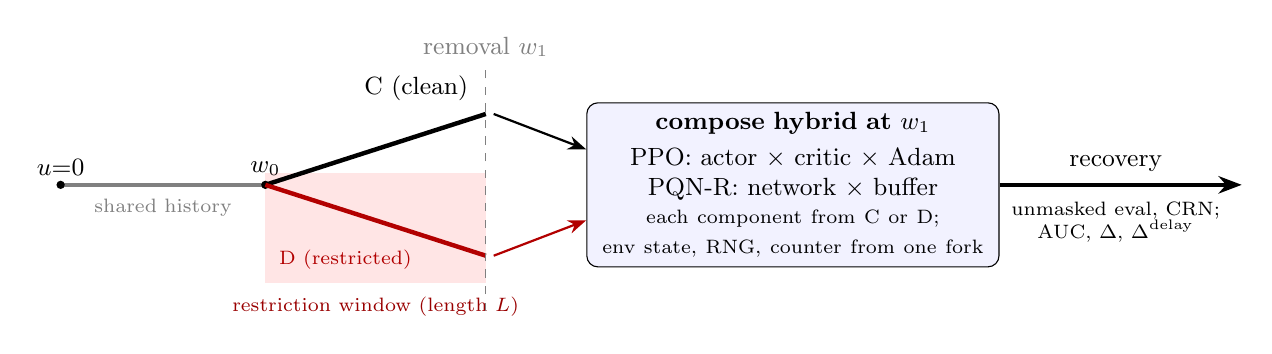
\begin{tikzpicture}[x=1cm,y=1cm,>=Stealth,font=\small]
  % restriction window shading (behind)
  \fill[red!10] (2.6,-1.25) rectangle (5.4,0.15);
  \node[red!60!black,font=\scriptsize,anchor=north] at (4.0,-1.3) {restriction window (length $L$)};
  % shared history
  \draw[line width=1.6pt,gray] (0,0) -- (2.6,0);
  \node[below,gray,font=\scriptsize] at (1.3,-0.05) {shared history};
  \fill (0,0) circle (1.5pt) node[above] {$u{=}0$};
  \fill (2.6,0) circle (1.5pt) node[above] {$w_0$};
  % forks
  \draw[line width=1.6pt] (2.6,0) -- (5.4,0.9);
  \draw[line width=1.6pt,red!70!black] (2.6,0) -- (5.4,-0.9);
  \node[anchor=south east] at (5.3,0.95) {C (clean)};
  \node[anchor=west,red!70!black,font=\scriptsize] at (2.65,-0.95) {D (restricted)};
  % removal
  \draw[dashed,gray] (5.4,-1.6) -- (5.4,1.5);
  \node[gray,anchor=south] at (5.4,1.5) {removal $w_1$};
  % surgery box
  \node[draw,rounded corners,fill=blue!5,align=center,text width=5.0cm] (box) at (9.3,0)
    {\textbf{compose hybrid at $w_1$}\\[2pt]
     PPO: actor $\times$ critic $\times$ Adam\\
     PQN-R: network $\times$ buffer\\[2pt]
     {\scriptsize each component from C or D;\\ env state, RNG, counter from one fork}};
  \draw[->,thick] (5.5,0.9) -- (box.west |- 0,0.45);
  \draw[->,thick,red!70!black] (5.5,-0.9) -- (box.west |- 0,-0.45);
  % recovery
  \draw[->,line width=1.2pt] (box.east) -- (15.0,0);
  \node[anchor=south] at (13.4,0.05) {recovery};
  \node[anchor=north,align=center,font=\scriptsize] at (13.4,-0.1) {unmasked eval, CRN;\\ AUC, $\Delta$, $\Ddel$};
\end{tikzpicture}
\caption{Protocol. A clean run C and a restricted run D share all state up to onset $w_0$. At removal $w_1$, hybrid agents are composed from components of either fork and trained without restriction. Every agent is evaluated on the full action set with common random numbers. Main effects compare the mean over hybrids holding the D version of a component with the mean over hybrids holding the C version.}
\label{fig:protocol}
\end{figure}

At removal we save the complete learner state of both forks and compose hybrids.
\begin{itemize}
\item \textbf{PPO} ($2^3$ factorial): actor parameters, critic parameters and Adam moments, each taken from C or D. Arms are labelled by the source of (actor, critic, optimizer); e.g.\ DDD is the damaged agent and CDD the damaged agent with a clean actor.
\item \textbf{PQN-R} ($2^2$): \emph{network} (parameters together with RAdam state; this assignment was pre-specified) and \emph{buffer} (all buffer arrays). The labels CC, DC, CD and DD give the sources of (network, buffer).
\end{itemize}
In both cases environment state, current observation, RNG and update counter come from a single fork, so the hybrids differ only in the transplanted components. A carrier's main effect is the mean over cells with its D version minus the mean over cells with its C version. We also report single transplants and rescues.

\subsection{Statistics and pre-registration}
All contrasts are paired by seed and reported as mean with a 95\% $t$-interval; $\sig$ marks intervals excluding 0. Seed counts are given for each experiment (4 to 32).

Our first analyses used percentile-bootstrap intervals over 4 seeds. These are anti-conservative, and all numbers reported here are the corrected $t$-intervals. The correction mattered once: the PPO delay-adjusted residual at $+250$ updates, which the bootstrap had marked as significant, is not (Section~\ref{sec:timing}).

\paragraph{Power.} Many early contrasts use $n=4$. Large effects (the actor effect, unlearning at removal) are tight even so, but nulls at $n=4$ are weak evidence. We handled this in three ways. (i) The two $n=4$ nulls that carry the paper's claims were re-tested with more seeds, under a pre-registration: the PPO component surgery ($n=12$, with equivalence tests) and the point-of-no-return test (8 fresh seeds). (ii) For every remaining $n=4$ null, Appendix Table~\ref{tab:power} reports the minimum detectable effect at 80\% power and the largest harm its interval excludes. (iii) We phrase those results as bounds (``deficits worse than $x$ are excluded''), not as absence of effect. One revision followed directly from this: with 12 seeds, a small critic effect that the 4-seed analysis missed became detectable (Section~\ref{sec:ppo}).

\paragraph{Confirmatory, exploratory and post-hoc evidence.} Every result in the paper has one of three statuses (Table~\ref{tab:status}).
\begin{itemize}
\item \emph{Confirmatory}: design, sample size, primary contrast, multiplicity correction and decision rule were committed to the public log before any data were generated.
\item \emph{Exploratory}: designed in advance, but without a committed analysis plan (Phases 1--5).
\item \emph{Post-hoc}: an analysis chosen after seeing the data.
\end{itemize}
Post-hoc analyses are labelled ``(post-hoc)'' wherever they appear. They never change or rescue a confirmatory verdict. They are reported only to qualify one (sensitivity of a margin, alternative baselines, minimum detectable effects), and the abstract and conclusion rest on confirmatory results. Pre-registration was introduced from the replay-purge experiments onward (Section~\ref{sec:ladder}). Two reviewer-response rounds (Phases 8 and 9) were pre-registered in full. Appendix~\ref{app:prov} lists the commit and manifest for each result.

\begin{table}[t]
\centering
\caption{Evidence status of the main claims. C = confirmatory (pre-registered before data; commit in parentheses), E = exploratory, P = post-hoc. $n$ = seeds.}
\label{tab:status}
\footnotesize
\resizebox{\linewidth}{!}{%
\begin{tabular}{llcl}
\toprule
claim & section & $n$ & status \\
\midrule
early restrictions cost only time; late restrictions cause unlearning (PPO, PQN, PQN-R) & \ref{sec:timing} & 4 & E \\
PPO late movement: $E_{\mathrm{damage}}$ (TOST $\pm3$) and $E_{\mathrm{plast}}$, fresh seeds & \ref{sec:timing} & 12 & C (Phase 9, 63a8f1d) \\
baselines B1--B3 for the other arms and learners (Table~\ref{tab:baselines}) & \ref{sec:timing}, App. & 4 & P \\
PPO surgery: actor, critic, optimizer main effects (Holm), TOST $\pm3$, Shapley & \ref{sec:ppo} & 12 & C (Phase 8, 8c62fe0); seeds 0--3 E \\
PPO ratio-neutral behaviour swap & \ref{sec:ppo} & 12 & C (Phase 8) \\
drift suppression, actor reset, fire restriction surgery & \ref{sec:ppo} & 4 & E \\
PQN-R network vs.\ buffer surgery & \ref{sec:pqnr} & 12 / 8 & E (assignment pre-specified) \\
PQN-R parameters vs.\ optimizer state & \ref{sec:pqnr} & 8 & C (Phase 8) \\
replay ladder, rungs 1--4 (primary contrasts) & \ref{sec:ladder} & 8--32 & C (864697e, 250cec4, 2559f2e, a873dc0) \\
rung 1 B$-$E, rung 3 ANOVA, rung 4 margin sensitivity & \ref{sec:ladder} & 8--32 & P \\
point-of-no-return gate (pilot) & \ref{sec:ponr} & 4 & C (ba1802f) \\
point of no return at $d=300$, TOST $\pm5$ & \ref{sec:ponr} & 8 & C (Phase 8) \\
replication at $d=300$ (pre-registered $n=32$, incomplete) & \ref{sec:ponr} & 16 & C, reported descriptively \\
removal-time predictors (pilot criteria R0--R3) & \ref{sec:ponr} & 16 & C (aabd1ae) \\
removal-time predictors vs.\ $A_{300}$ (pre-registered $n=32$, incomplete) & \ref{sec:ponr} & 16 & C, reported descriptively \\
outcome reliability; pooling across studies & \ref{sec:ponr} & -- & P \\
generalization: Asterix, reward flip, $2\times256$ & \ref{sec:general} & 8 & C (Phase 8) \\
Asterix with the reward-flip deficit & \ref{sec:general} & 4 & C (Phase 9; $n$ cut from 8) \\
gap at removal vs.\ total damage across settings & \ref{sec:general} & -- & P \\
minimum detectable effects (Table~\ref{tab:power}) & App. & -- & P \\
\bottomrule
\end{tabular}}
\end{table}

%=====================================================================
\section{Early restrictions cost time; late restrictions cause unlearning}\label{sec:timing}
%=====================================================================

\begin{figure}[t]
\centering
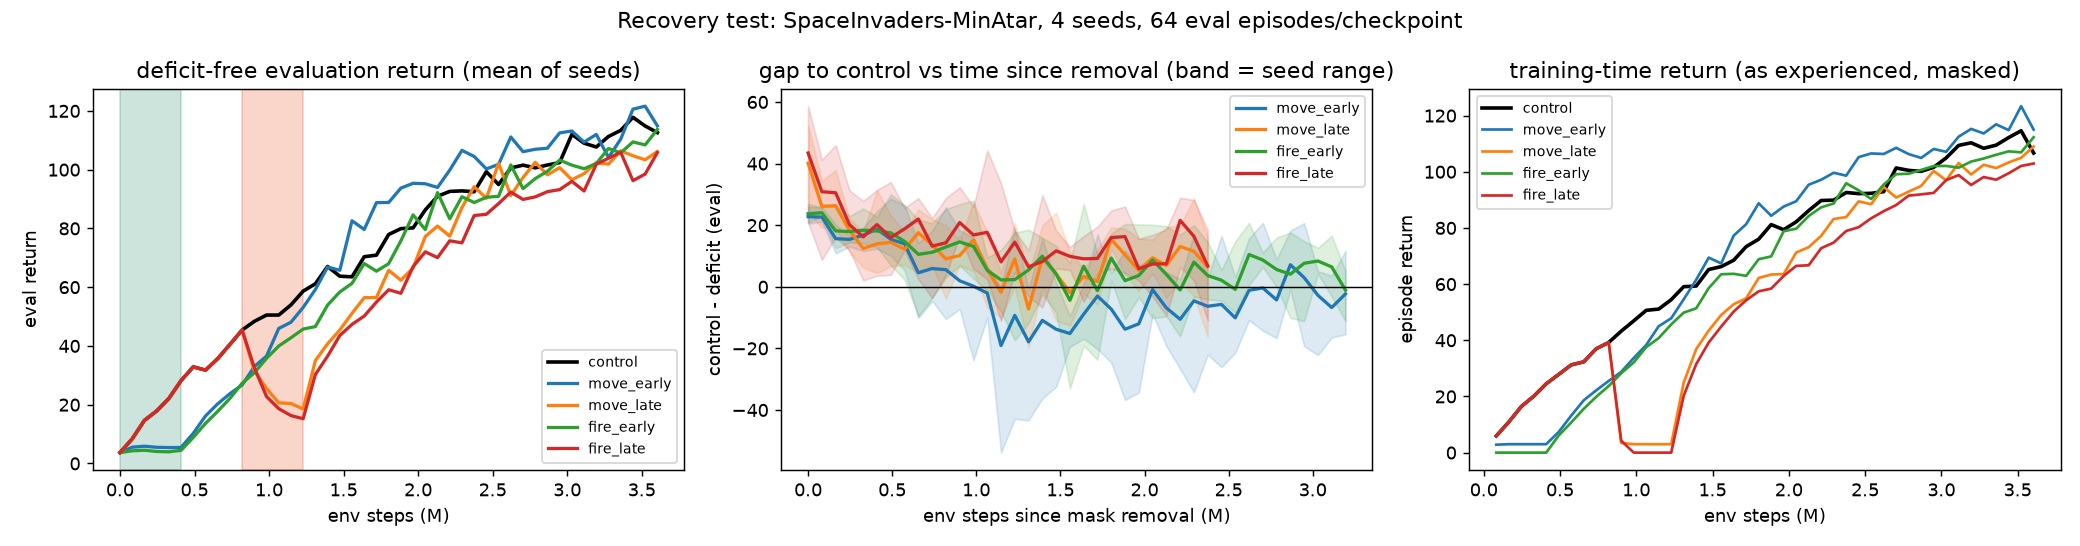
\includegraphics[width=\linewidth]{figures/recovery_all.png}
\caption{PPO recovery test on SpaceInvaders-MinAtar, 4 seeds, 64 evaluation episodes per checkpoint. \textbf{Left:} evaluation with the full action set (shaded: early and late windows). \textbf{Middle:} control $-$ arm gap against time since removal (the repository's sign convention; positive = arm behind). \textbf{Right:} training return as experienced under the restriction. Early-restricted agents never had competence to lose. Late-restricted agents collapse below their competence at onset and then catch up.}
\label{fig:recovery}
\end{figure}

\begin{table}[t]
\centering
\caption{PPO recovery test ($n=4$, paired 95\% $t$-intervals). $\Delta$ = restricted $-$ control at the same update; $\Ddel$ = restricted $-$ control $L{=}50$ updates earlier. Negative = harm. At removal, $\Ddel$ is the change in competence during the window.}
\label{tab:ppo_recovery}
\small
\begin{tabular}{llccc}
\toprule
arm & readout & update & $\Delta$ & $\Ddel$ \\
\midrule
move, early $[0,50)$ & at removal & 50  & $-22.8\ci{-26.8}{-18.7}\sig$ & $+1.8\ci{+0.9}{+2.6}\sig$ \\
                     & $+50$       & 100 & $-17.0\ci{-24.8}{-9.1}\sig$  & $+0.1\ci{-7.5}{+7.6}$ \\
                     & $+250$      & 300 & $+6.6\ci{-10.7}{+23.9}$      & $+16.4\ci{+2.1}{+30.6}\sig$ \\
move, late $[100,150)$ & at removal & 150 & $-40.1\ci{-58.7}{-21.6}\sig$ & $-26.9\ci{-45.6}{-8.1}\sig$ \\
                       & $+50$       & 200 & $-13.6\ci{-24.9}{-2.3}\sig$  & $-3.3\ci{-15.0}{+8.5}$ \\
                       & $+250$      & 400 & $-7.2\ci{-13.2}{-1.3}\sig$   & $+2.0\ci{-0.1}{+4.1}$ \\
\midrule
fire, early $[0,50)$ & at removal & 50  & $-23.7\ci{-28.1}{-19.3}\sig$ & $+0.8\ci{-0.2}{+1.7}$ \\
                     & $+250$      & 300 & $-5.5\ci{-18.1}{+7.2}$       & $+4.3\ci{-19.8}{+28.4}$ \\
fire, late $[100,150)$ & at removal & 150 & $-43.4\ci{-70.9}{-15.9}\sig$ & $-30.2\ci{-41.3}{-19.1}\sig$ \\
                       & $+250$      & 400 & $-6.9\ci{-17.9}{+4.1}$       & $+2.4\ci{-3.6}{+8.3}$ \\
\bottomrule
\end{tabular}
\end{table}

\paragraph{PPO.}
Table~\ref{tab:ppo_recovery} and Figure~\ref{fig:recovery} show the timing pattern for PPO.

\emph{Early windows.} An early restriction leaves the agent far behind the control at removal ($\Delta=-22.8$), but this is entirely lost time: competence did not fall during the window ($\Ddel=+1.8$). By $+250$ updates the early-restricted agent is ahead of a control 50 updates younger ($\Ddel=+16.4\ci{+2.1}{+30.6}$). Some learning happened during the restriction.

\emph{Late windows.} A late restriction causes \emph{unlearning}: unmasked evaluation falls from 45.4 at onset to 18.5 at removal ($\Ddel=-26.9$ for movement, $-30.2$ for fire). It is then followed by fast relearning. After 250 updates (2.05M steps) the raw deficit ($-7.2$) is fully explained by lost time ($\Ddel=+2.0\ci{-0.1}{+4.1}$; fire $+2.4\ci{-3.6}{+8.3}$).

\emph{Pilots.} Earlier onset sweeps with 400k-step windows at five onsets showed the same direction: later was worse at a fixed final budget. No window showed detectable damage beyond lost time. With corrected $t$-intervals, the latest action-mask onset gave $\Ddel=-5.4\ci{-11.6}{+0.8}$ and observation noise at onset 0.3 gave $-2.8\ci{-6.8}{+1.1}$.

\begin{table}[t]
\centering
\caption{PQN and PQN-R recovery (100k buffer), movement restriction ($n=4$, $\epsilon=0.05$ evaluation). Restriction length $L=100$ updates (409{,}600 steps); AUC averages checkpoints $+10$ to $+900$ (early) or $+650$ (late) after removal. Negative = harm.}
\label{tab:pqn_recovery}
\small
\begin{tabular}{lllcc}
\toprule
agent & window & readout & $\Delta$ & $\Ddel$ \\
\midrule
PQN   & early $[0,100)$   & at removal & $-19.0\ci{-21.1}{-16.9}\sig$ & $+2.4\ci{-1.0}{+5.9}$ \\
      &                   & AUC        & $-0.5\ci{-4.5}{+3.5}$        & $+6.4\ci{+2.4}{+10.5}\sig$ \\
      & late $[250,350)$  & at removal & $-58.3\ci{-70.6}{-45.9}\sig$ & $-43.2\ci{-67.3}{-19.2}\sig$ \\
      &                   & AUC        & $-4.6\ci{-7.2}{-2.0}\sig$    & $-1.4\ci{-3.5}{+0.7}$ \\
\midrule
PQN-R & early $[0,100)$   & at removal & $-7.4\ci{-16.4}{+1.5}$       & $+2.8\ci{-1.6}{+7.2}$ \\
      &                   & AUC        & $-2.7\ci{-5.2}{-0.1}\sig$    & $+2.7\ci{-0.2}{+5.5}$ \\
      & late $[250,350)$  & at removal & $-23.4\ci{-32.5}{-14.4}\sig$ & $-23.4\ci{-26.8}{-20.0}\sig$ \\
      &                   & $+100$     & $-14.4\ci{-22.5}{-6.3}\sig$  & $-5.7\ci{-12.0}{+0.5}$ \\
      &                   & AUC        & $-8.6\ci{-11.6}{-5.6}\sig$   & $-4.3\ci{-7.0}{-1.6}\sig$ \\
      &                   & $+650$     & $-3.2\ci{-18.4}{+12.0}$      & $-0.2\ci{-7.7}{+7.3}$ \\
\bottomrule
\end{tabular}
\end{table}

\paragraph{PQN and PQN-R.}
The same pattern replicates with value-based learners whose meaning-matched onset lies at a different update (Table~\ref{tab:pqn_recovery}; Figure~\ref{fig:pqn_recovery} in the appendix).
\begin{itemize}
\item \emph{Early restrictions} produce no unlearning, and the agents recover at least as fast as a delayed control: PQN's delay-adjusted AUC is $+6.4\ci{+2.4}{+10.5}$.
\item \emph{Late restrictions} cause severe unlearning. The restricted PQN agent's evaluation return at removal is 3.6, against 61.8 for the control, and its restriction-era policy is far below its own competence at onset.
\item \emph{After removal}, PQN recovers to within lost time (delay-adjusted AUC $-1.4\ci{-3.5}{+0.7}$). PQN-R is the one learner with a recovery cost beyond lost time: delay-adjusted AUC $-4.3\ci{-7.0}{-1.6}$. The cost is transient; by $+650$ updates the delay-adjusted difference is $-0.2\ci{-7.7}{+7.3}$.
\end{itemize}

\paragraph{Declared estimands on fresh seeds (confirmatory).}
The results above use the primary estimand, but on exploratory seeds. We therefore pre-registered a confirmatory test of both declared estimands (Section~\ref{sec:estimands}) on 12 fresh seeds (200--211), for the PPO late movement restriction with $K=250$ (Table~\ref{tab:estimands}).
\begin{itemize}
\item \textbf{Damage beyond lost time ($E_{\mathrm{damage}}$, primary).} The estimate is $+1.9\ci{-0.7}{+4.4}$, so the restricted agent ends slightly \emph{ahead} of a paused control. The pre-registered TOST against $\pm3$ is \emph{inconclusive} ($p=0.17$). Its harmful side is rejected decisively: a mean below $-3$ is rejected at $p=0.0007$, and the interval excludes harm beyond $-0.7$. Equivalence fails only because a \emph{benefit} larger than $+3$ cannot be excluded. Within 250 updates, therefore, damage beyond lost time larger than about 0.7 AUC points is excluded, and the direction of any residual is open.
\item \textbf{Relearning from equal competence ($E_{\mathrm{plast}}$).} $+14.2\ci{+10.9}{+17.5}\sig$, positive in 12/12 seeds. Restricted agents relearn faster than the clean agent first learned from the same competence: a savings effect, not slower relearning.
\item \textbf{Total cost ($E_{\mathrm{total}}$, descriptive).} $-8.9\ci{-11.1}{-6.6}\sig$. The practitioner still pays for the lost time.
\end{itemize}
The three numbers differ in sign because they answer different questions, not because the conclusion is ambiguous. The deficit costs time ($E_{\mathrm{total}}<0$), it does not detectably cost more than that time ($E_{\mathrm{damage}}$, with harm $>0.7$ excluded), and it does not slow relearning ($E_{\mathrm{plast}}>0$).
\emph{Other arms and learners (post-hoc, $n=4$).} Appendix Table~\ref{tab:baselines} applies the same three counterfactuals to the exploratory runs. In every late arm the ordering is $E_{\mathrm{total}}<E_{\mathrm{damage}}<E_{\mathrm{plast}}$, and $E_{\mathrm{plast}}$ is positive. $E_{\mathrm{damage}}$ is detectably negative only for PQN-R ($-4.3\sig$), the one learner with transient damage beyond lost time. These comparisons are descriptive.

\begin{table}[t]
\centering
\caption{Confirmatory test of the declared estimands (pre-registered, Phase 9). PPO, late movement restriction $[100,150)$, 12 fresh seeds (200--211), AUC over $k=10..250$ after removal, paired 95\% $t$-intervals. Negative = restricted agent worse. $t^\star$: mean 52 updates (range 30--90). Source: \url{p9_estimands-analysis.md}.}
\label{tab:estimands}
\small
\resizebox{\linewidth}{!}{%
\begin{tabular}{llllc}
\toprule
estimand & question & counterfactual & estimate & pre-registered decision \\
\midrule
$E_{\mathrm{damage}}$ (primary) & damage beyond lost time & pause, $C(w_1+k-L)$ & $+1.9\ci{-0.7}{+4.4}$ & inconclusive (TOST $\pm3$, $p=0.17$); harm $<-3$ rejected, $p=0.0007$ \\
$E_{\mathrm{plast}}$ & slower relearning from equal competence & competence-matched, $C(t^\star+k)$ & $+14.2\ci{+10.9}{+17.5}\sig$ & savings (12/12 seeds) \\
$E_{\mathrm{total}}$ & total cost incl.\ lost time & same update, $C(w_1+k)$ & $-8.9\ci{-11.1}{-6.6}\sig$ & descriptive \\
\bottomrule
\end{tabular}}
\end{table}

\paragraph{Summary.}
The timing pattern is the reverse of a critical period. In our data, damage beyond lost time appeared only after something had been learned that could be lost, and even then it was largely relearned. Removing movement actions after the agent has learned to dodge is what hurts.

%=====================================================================
\section{In PPO, the damage lives mainly in the actor}\label{sec:ppo}
%=====================================================================

\begin{figure}[t]
\centering
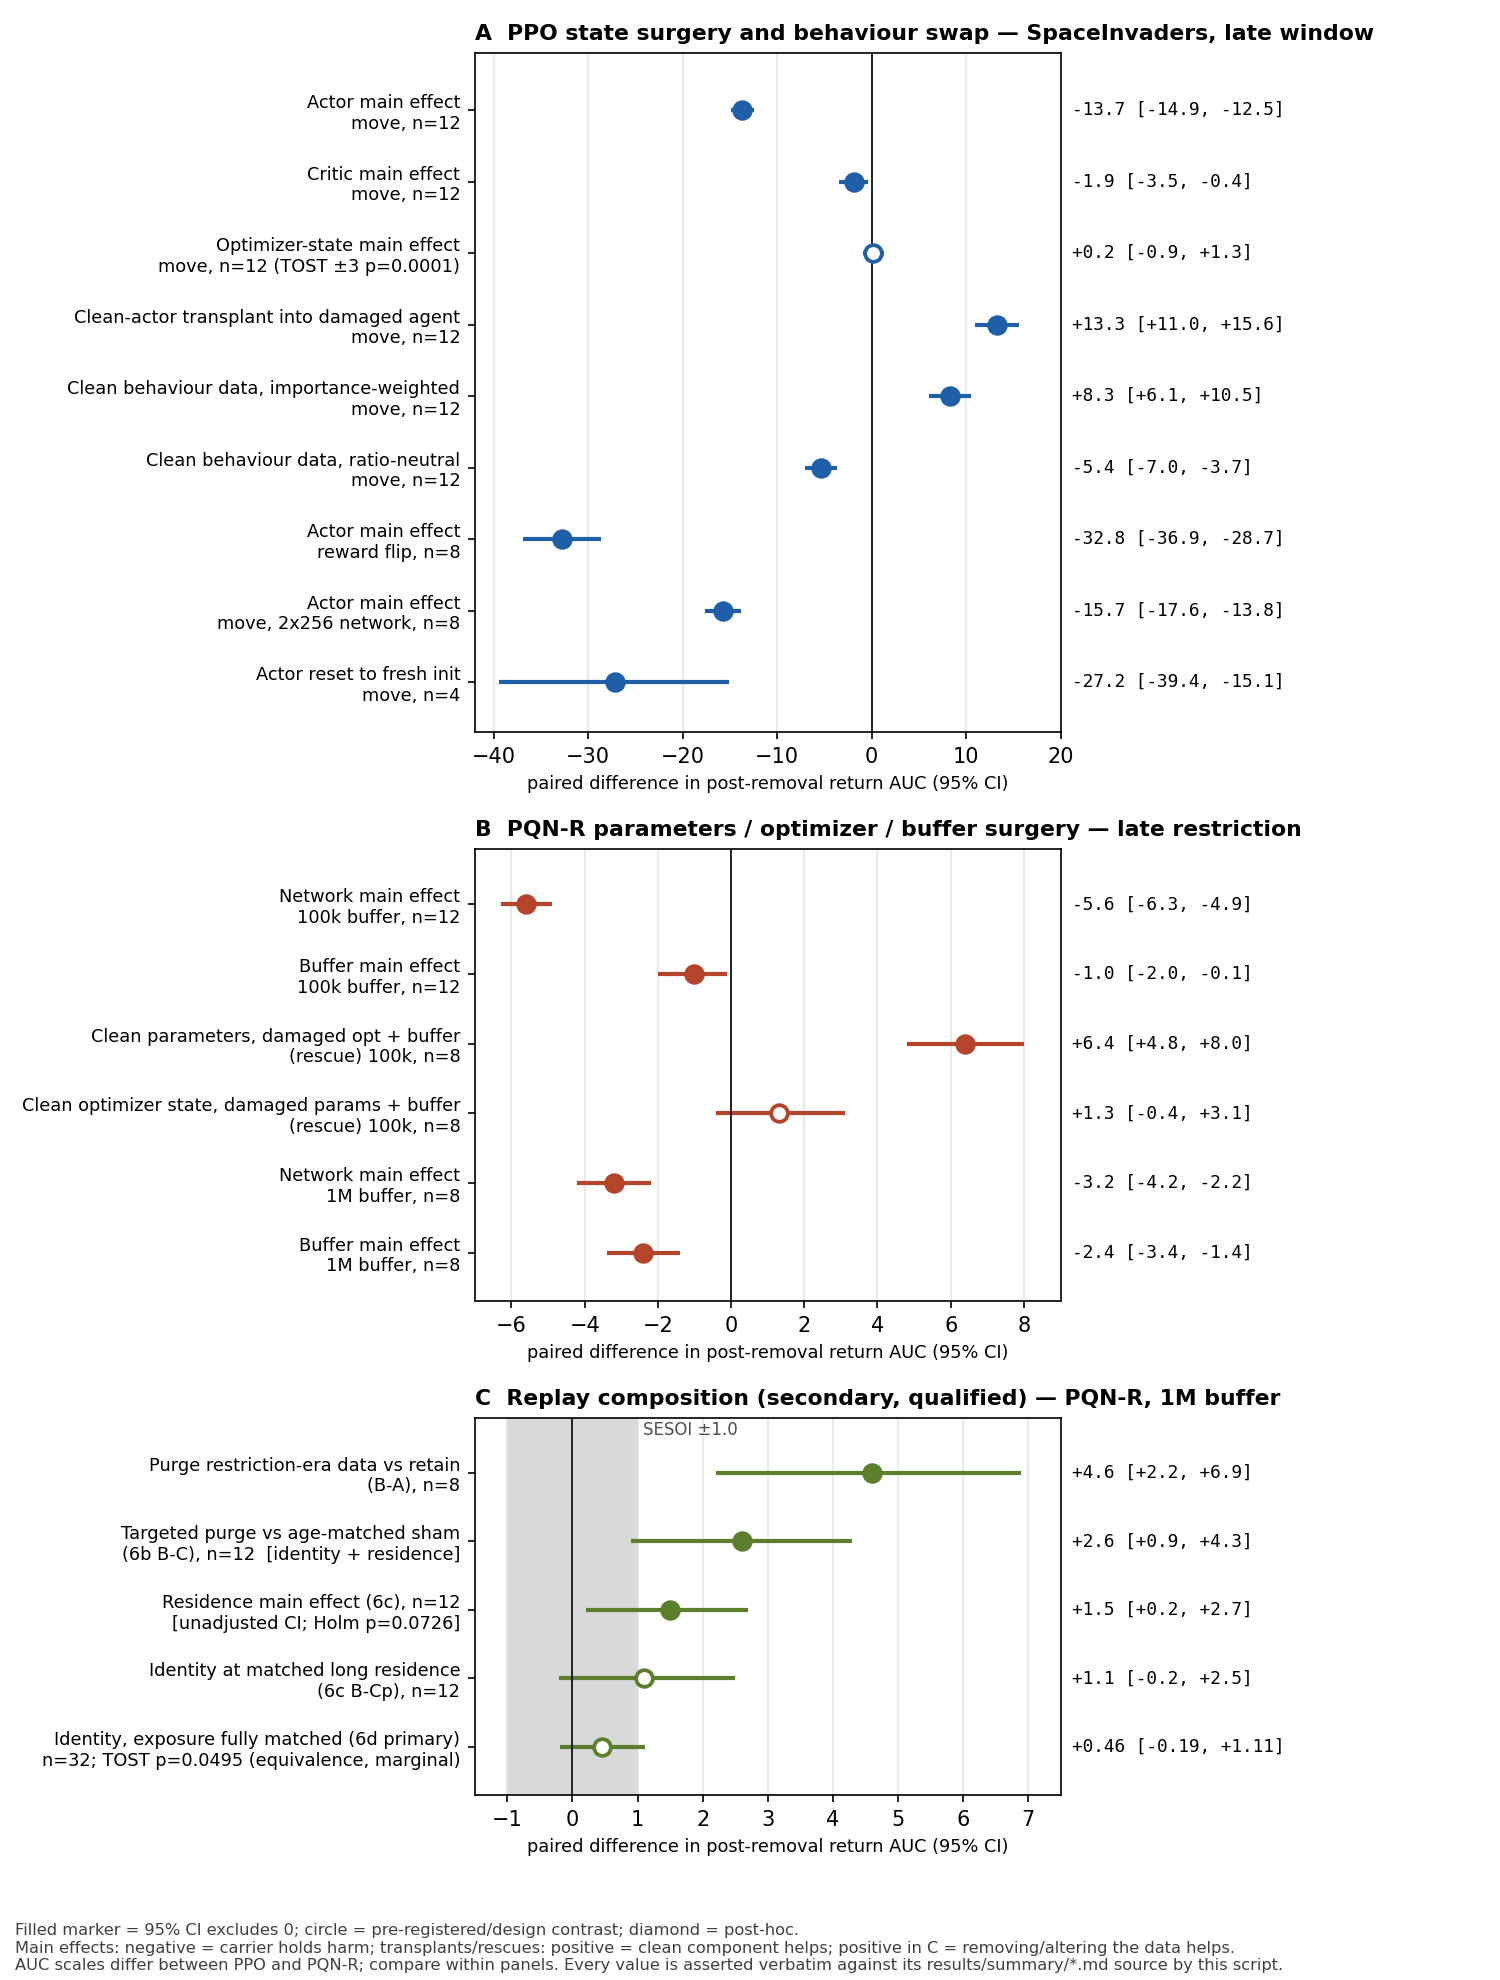
\includegraphics[width=0.78\linewidth]{figures/causal_summary.png}
\caption{Summary of the causal contrasts (paired differences in post-removal return AUC, 95\% $t$-intervals). \textbf{A}: PPO actor/critic/optimizer surgery ($n=12$), clean-actor transplant, behaviour swap with and without importance weighting, the actor effect under the reward-flip deficit, and actor reset. \textbf{B}: PQN-R network vs.\ buffer surgery, and the parameter vs.\ optimizer-state split. \textbf{C}: the replay ladder, with the pre-registered equivalence margin $\pm1$ (grey). Filled markers: interval excludes 0; diamond: post-hoc. For main effects, negative values mean the component holds harm; for transplants and rescues, positive values mean the clean component helps; positive values in C mean removing or altering the data helps. AUC scales differ between PPO and PQN-R.}
\label{fig:summary}
\end{figure}

\begin{table}[t]
\centering
\caption{PPO $2^3$ state surgery at removal of the late movement restriction ($n=12$: seeds 0--3 exploratory, seeds 4--11 pre-registered replication). Recovery AUC over 150 updates. Main effects are D$-$C averages over the other two components (Holm across the three). Shapley values are an exact additive decomposition of the total (they sum to it per seed), and the share is the ratio of means. Arm labels give the sources of (actor, critic, optimizer). Rows marked $^\dagger$ come from Phase 4 ($n=4$). Source: \url{p8_ppo_surgery_n12-analysis.md}.}
\label{tab:ppo_surgery}
\small
\resizebox{\linewidth}{!}{%
\begin{tabular}{lccc}
\toprule
contrast & AUC & $+10$ & Shapley value (share) \\
\midrule
total damage DDD $-$ CCC & $-15.1\ci{-17.2}{-13.0}\sig$ & $-28.4\ci{-33.4}{-23.4}\sig$ & $-15.1$ (100\%) \\
\midrule
actor main effect   & $-13.7\ci{-14.9}{-12.5}\sig$ & $-18.5\ci{-23.2}{-13.9}\sig$ & $-13.6\ci{-15.0}{-12.2}\sig$ (90\%) \\
critic main effect  & $-1.9\ci{-3.5}{-0.4}\sig$ & $-4.4\ci{-6.4}{-2.5}\sig$ & $-1.8\ci{-3.2}{-0.4}\sig$ (12\%) \\
optimizer (Adam) main effect & $+0.2\ci{-0.9}{+1.3}$ & $-4.9\ci{-6.9}{-3.0}\sig$ & $+0.3\ci{-0.9}{+1.5}$ ($-2$\%) \\
\quad actor, fresh seeds 4--11 only ($n=8$) & $-14.2\ci{-16.0}{-12.4}\sig$ & & \\
\midrule
damaged actor only, DCC $-$ CCC   & $-13.3\ci{-16.2}{-10.4}\sig$ & & \\
clean actor into damaged agent, CDD $-$ DDD & $+13.3\ci{+11.0}{+15.6}\sig$ & & \\
clean actor transplant vs.\ clean, CDD $-$ CCC & $-1.8\ci{-4.5}{+0.9}$ & & \\
clean critic into damaged agent, DCD $-$ DDD & $+3.0\ci{+0.8}{+5.3}\sig$ & & \\
actor reset to fresh init, vs.\ DDD$^\dagger$ & $-27.2\ci{-39.4}{-15.1}\sig$ & & \\
actor + optimizer reset, vs.\ DDD$^\dagger$ & $-24.5\ci{-26.8}{-22.1}\sig$ & & \\
\midrule
\multicolumn{4}{l}{\emph{behaviour swap for the first 10 updates} ($n=12$)} \\
clean behaviour, importance-weighted, DDD+bC $-$ DDD & $+8.3\ci{+6.1}{+10.5}\sig$ & $+11.8\ci{+7.0}{+16.6}\sig$ & \\
clean behaviour, ratio-neutral, DDD+bCr $-$ DDD & $-5.4\ci{-7.0}{-3.7}\sig$ & $-18.0\ci{-22.4}{-13.5}\sig$ & \\
damaged behaviour, importance-weighted, CCC+bD $-$ CCC & $-9.4\ci{-14.7}{-4.2}\sig$ & $-26.8\ci{-34.4}{-19.1}\sig$ & \\
damaged behaviour, ratio-neutral, CCC+bDr $-$ CCC & $-2.5\ci{-6.6}{+1.7}$ & $-11.7\ci{-25.0}{+1.5}$ & \\
\bottomrule
\end{tabular}}
\end{table}

\paragraph{Factorial surgery.}
Table~\ref{tab:ppo_surgery} decomposes the 150-update recovery deficit after the late movement restriction (total $-15.1$ AUC, $n=12$). The first four seeds were exploratory. The eight further seeds, the multiplicity correction, the equivalence margins and the Shapley attribution were pre-registered before any of the new data were generated.
\begin{itemize}
\item \textbf{Actor.} The actor main effect is $-13.7\ci{-14.9}{-12.5}$, and it replicates on the fresh seeds alone ($-14.2\ci{-16.0}{-12.4}$, $n=8$). Main-effect ``shares'' of a non-additive factorial do not partition the total, so we attribute with exact Shapley values instead. These sum to the total per seed by construction. The actor's Shapley value is $-13.6\ci{-15.0}{-12.2}$, \textbf{90\%} of the damage, negative in 12/12 seeds. A damaged actor alone in an otherwise clean agent reproduces almost all of the damage ($-13.3$), and a clean actor transplanted into the damaged agent rescues $+13.3$. After the transplant, the hybrid is statistically indistinguishable from the clean agent ($-1.8\ci{-4.5}{+0.9}$).
\item \textbf{Critic.} With 12 seeds the critic shows a small, detectable contribution: main effect $-1.9\ci{-3.5}{-0.4}$ (Holm $p=0.038$), Shapley share 12\%, clean-critic rescue $+3.0\ci{+0.8}{+5.3}$. The effect is transient. It is $-4.4$ at $+10$ updates and $-0.2\ci{-3.9}{+3.6}$ at $+150$. It is not equivalent to zero within the pre-registered $\pm3$ margin (TOST $p=0.08$). Our 4-seed analysis had reported no detectable critic effect, which was a power limitation.
\emph{How the main effect and the Shapley value relate.} Both summarize the same four critic swaps (damaged minus clean critic, in each of the four actor $\times$ optimizer backgrounds). The main effect weights the four swaps equally. The Shapley value weights them $\tfrac13,\tfrac16,\tfrac16,\tfrac13$, so the all-clean and all-damaged backgrounds count more. The two coincide when there are no interactions, and here they nearly do ($-1.9$ vs.\ $-1.8$). Only the Shapley values add up to the total ($90\%+12\%-2\%=100\%$), which is why we use them for shares. Both are significantly negative.
Throughout the paper, ``transient'' describes the time course: the critic's contribution is concentrated in the first updates after removal and undetectable by $+150$. It does not mean the AUC effect is unreliable. We therefore call the critic a \emph{minor, transient carrier}, neither uninvolved nor equivalent to zero. The same pattern recurs with the wider network (main effect $-2.5$, Shapley 15\%; Section~\ref{sec:general}). Under the reward flip, where the actor's share is about 100\%, the critic was not detectable ($+1.2$).
\item \textbf{Optimizer state.} No damage was detected in the Adam moments, and their contribution is bounded. The main effect $+0.2\ci{-0.9}{+1.3}$ is statistically equivalent to zero within $\pm3$ AUC (TOST $p=0.0001$). A brief $-4.9$ dip at $+10$ updates, when damaged moments drive the first steps, is fully washed out by $+50$.
\item \textbf{Fire restriction.} The same holds for the distinct fire restriction ($n=4$): total $-17.4\ci{-31.2}{-3.6}$, clean-actor transplant $+12.9\ci{+1.3}{+24.5}$.
\end{itemize}

\paragraph{The damaged actor is far better than a fresh one.}
Re-initializing the actor while keeping the critic and optimizer is \emph{much worse} than keeping the damaged actor: $-27.2\ci{-39.4}{-15.1}$ for movement and $-23.4\ci{-35.6}{-11.1}$ for fire. Resetting the actor's Adam moments as well changes little ($-24.5$).

A fresh actor in this setting learns no faster than a from-scratch agent. It reaches 26.9 after 50 updates, against 28.2 for the from-scratch control at the same point. The damaged actor therefore retains most of its useful structure, and is not a plasticity-impaired network that a reset would help. This contrasts with the success of resets under the primacy bias \citep{nikishin2022primacy}.

\paragraph{Does preventing unlearning help? No.}
We suppressed policy drift during the restriction in two ways (Appendix Figure~\ref{fig:drift}):
\begin{itemize}
\item \emph{F}: freeze the actor's hidden layers, leaving the logit head trainable;
\item \emph{A}: anchor the policy to the onset policy with a KL penalty ($\beta=1$).
\end{itemize}
Both largely prevented the collapse. Evaluation at removal improved by $+20.1\ci{+8.2}{+32.0}$ (F) and $+21.1\ci{+13.1}{+29.0}$ (A), and representation drift fell. Yet neither detectably improved recovery AUC: $+1.1\ci{-3.4}{+5.7}$ and $-0.0\ci{-1.8}{+1.7}$. Both stayed as far behind the clean agent as the unprotected one ($-13.2$, $-14.4$).

Unlearned competence is relearned so quickly that protecting it buys nothing. What the clean actor holds that the damaged and the protected actors lack is the \emph{progress} made during the window. This is consistent with Section~\ref{sec:timing}: the persistent cost is lost time, and the actor is where most of that time's learning is stored.

\paragraph{The actor--experience loop.}
On-policy data is generated by the actor, so ``data damage'' in PPO cannot be separated from the actor by surgery on stored arrays alone. We swapped the behaviour policy for the first $K=10$ post-removal updates. In the original design (exploratory, now replicated at $n=12$), data from the clean actor rescued the damaged agent ($+8.3$), and data from the damaged actor harmed a clean one ($-9.4$). Clean data from a \emph{different} seed had no detectable effect ($+2.4\ci{-5.6}{+10.4}$, $n=4$). Neither did a tempered version of the agent's own policy, matched in KL distance from the clean policy ($-5.1\ci{-14.3}{+4.1}$).

That design is confounded: PPO's importance ratio $\pi_\theta/\pi_b$ now involves a foreign behaviour policy, and the clip fraction rises from 0.09 to 0.34. We therefore pre-registered \emph{ratio-neutral} arms, in which the stored log-probability is the learner's own. PPO then sees the same states, actions and rewards from $\pi_b$, but its ratio starts at 1 and carries no importance weighting. The result is unambiguous. Without importance weights, clean behaviour data \emph{harm} the damaged learner ($-5.4\ci{-7.0}{-3.7}$, Holm $p<10^{-4}$), and damaged data no longer detectably harm a clean one ($-2.5\ci{-6.6}{+1.7}$). The importance-weighted and ratio-neutral versions differ by $+13.6\ci{+11.5}{+15.7}$.

What the importance weights add is a pull toward the behaviour policy. During the swap, the KL divergence from the behaviour policy to the learner is $0.13$--$0.18$ with importance weighting and $0.76$--$1.07$ without it. With a clean behaviour policy, the original swap amounts to a brief off-policy distillation of the clean \emph{actor}. The ratio-neutral clip fraction (0.20--0.23) shows that large policy changes still occur, but they come from the learner's own updates on unfamiliar data. We conclude that clean data content alone does not repair the damage. The benefit of the original swap is actor information transmitted through the update rule, which places the carrier in the actor again. Even the ratio-neutral arm is not a pure-data intervention, since it applies on-policy updates to off-policy actions, so no PPO arm cleanly isolates data content from the update.

%=====================================================================
\section{In PQN-R, the network carries the damage; the buffer mediates}\label{sec:pqnr}
%=====================================================================

\begin{table}[t]
\centering
\caption{PQN-R network $\times$ buffer surgery after the late movement restriction. Network = parameters + RAdam state (separated in the text: parameters carry 87\% of the network rescue). Recovery AUC over $+10$ to $+650$ updates; $\epsilon=0.05$ evaluation. Arm labels give the sources of (network, buffer). The ``gone'' phase starts once no restriction-era transition remains in any buffer. $^{\dagger}$For the 100k buffer, phase contrasts use the 8 seeds (4--11) with per-slot age tags.}
\label{tab:pqnr}
\small
\begin{tabular}{lcc}
\toprule
contrast & 100k buffer ($n=12$) & 1M buffer ($n=8$) \\
\midrule
total damage DD $-$ CC & $-6.7\ci{-8.0}{-5.3}\sig$ & $-5.6\ci{-7.0}{-4.2}\sig$ \\
parameter transfer DC $-$ CC & $-4.6\ci{-6.1}{-3.0}\sig$ & $-2.6\ci{-3.6}{-1.6}\sig$ \\
data transfer CD $-$ CC & $+0.0\ci{-1.0}{+1.0}$ & $-1.7\ci{-3.3}{-0.2}\sig$ \\
network main effect & $-5.6\ci{-6.3}{-4.9}\sig$ (84\%) & $-3.2\ci{-4.2}{-2.2}\sig$ (57\%) \\
buffer main effect & $-1.0\ci{-2.0}{-0.1}\sig$ (16\%) & $-2.4\ci{-3.4}{-1.4}\sig$ (43\%) \\
interaction & $-2.1\ci{-4.5}{+0.2}$ & $-1.3\ci{-3.2}{+0.6}$ \\
\midrule
restriction-era share of buffer at removal & 0.96 & 0.41 \\
restriction-era data gone after & $+25$ updates & $+245$ updates \\
buffer main effect, ``gone'' phase$^{\dagger}$ & $-0.9\ci{-2.3}{+0.4}$ & $-2.9\ci{-4.1}{-1.8}\sig$ \\
total damage, ``gone'' phase$^{\dagger}$ & $-6.0\ci{-8.1}{-4.0}\sig$ & $-7.1\ci{-9.2}{-4.9}\sig$ \\
\midrule
eval at removal, D vs.\ C network & 4.2 vs.\ 32.0 ($-87\%$) & 14.1 vs.\ 27.8 ($-50\%$) \\
\bottomrule
\end{tabular}
\end{table}

\begin{figure}[t]
\centering
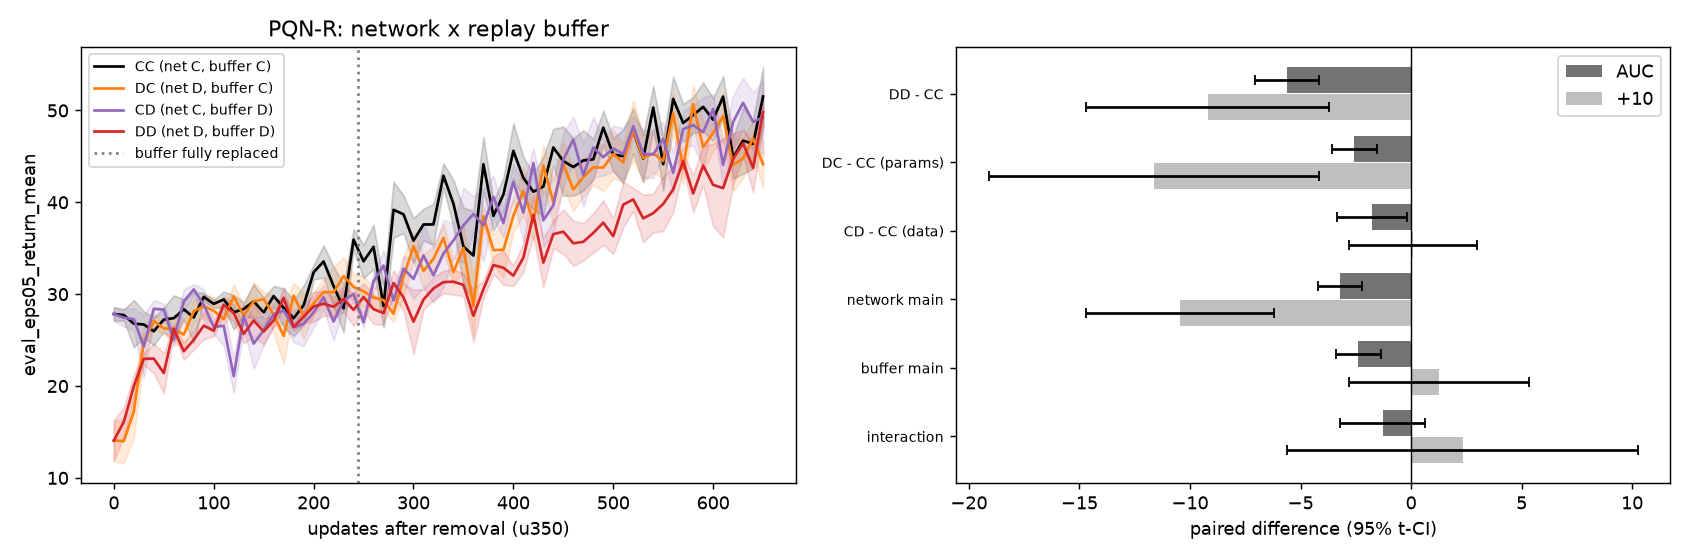
\includegraphics[width=\linewidth]{figures/p6_surgery_pqnr1m_n8.png}
\caption{PQN-R network $\times$ buffer surgery with a 1M buffer ($n=8$). \textbf{Left:} recovery curves (dotted line: the last restriction-era transition leaves the buffer at $+245$). \textbf{Right:} paired contrasts for AUC and for the $+10$ readout. A damaged network hurts recovery throughout. The damaged buffer's harm is concentrated \emph{after} its restriction-era data is gone.}
\label{fig:pqnr1m}
\end{figure}

PQN-R lets us separate parameters from stored data directly. With the default 100k buffer the network dominates (Table~\ref{tab:pqnr}): 84\% of the damage, parameter transfer $-4.6$, data transfer $+0.0\ci{-1.0}{+1.0}$. The result is consistent across seeds: the network effect is negative in 12/12 seeds, with a prediction interval for a new seed of $[-8.1,-3.1]$. Restriction-era data fill 96\% of the 100k buffer at removal and are fully overwritten within 25 updates. The damage that remains after that point ($-6.0$) is a network effect. In a $2\times2$ design, main effects coincide with exact Shapley values and sum to the total, so these percentages do form a partition, unlike the PPO main-effect shares in our earlier analysis.

\paragraph{Parameters, not optimizer state (pre-registered).}
Network surgery moves parameters and RAdam moments together. To separate them we ran a pre-registered $2\times2$ (parameters $\times$ optimizer state) at the damaged buffer ($n=8$, 100k buffer). Its DDD cell reproduced the earlier damaged arm bit for bit in all 8 seeds. Clean parameters with the damaged optimizer state and buffer rescue $+6.4\ci{+4.8}{+8.0}$ AUC (Holm $p=10^{-4}$), 87\% of the full network rescue ($+7.3$). Clean optimizer state with damaged parameters rescues $+1.3\ci{-0.4}{+3.1}$ (Holm $p=0.12$). The optimizer main effect in the $2\times2$ is small but detectable ($+1.1\ci{+0.4}{+1.9}$), and it is concentrated in a transient interaction: clean parameters paired with stale RAdam moments briefly crash at $+10$ updates (11.1 vs.\ 29.9 with matched moments), then recover by $+150$. The PQN-R network carrier is therefore its parameters, as in PPO, where the actor parameters carry the damage and Adam state is equivalent to zero.

\paragraph{The buffer as a mediator.}
A 1M buffer is not simply a longer memory. It holds restriction-era data for 245 updates after removal (41\% of slots at removal), and it also dilutes the restriction while it is happening: the collapse at removal is $-50\%$ rather than $-87\%$.

With 1M slots the buffer main effect becomes significant ($-2.4\ci{-3.4}{-1.4}$, 43\%). Its time course rules out the simplest reading, in which the old data is consumed and directly causes worse targets. The buffer effect is $-1.4\ci{-2.7}{-0.0}$ while restriction-era data are present ($+10$ to $+150$), and $-2.9\ci{-4.1}{-1.8}$ \emph{after they are gone} ($+250$ to $+650$; Figure~\ref{fig:pqnr1m}).

Training on the restricted buffer during the first 245 updates leaves its mark in the network, and that mark outlasts the data. The buffer shapes the damage; it does not store it.

%=====================================================================
\section{A replay ladder: the data-identity effect shrinks under matching}\label{sec:ladder}
%=====================================================================

Is there something specific about the \emph{identity} of restriction-era transitions, or do apparent data effects reflect how much fresh data enters the buffer and how long it stays? We ran four increasingly matched experiments, all on PQN-R with a 1M buffer. All replacement data are real transitions newly collected with a fixed protocol: a frozen clean actor (the clean fork's parameters at removal), $\epsilon=0.05$, the full action set, fresh environments and a separate RNG stream. The pool is collected once per seed and frozen. Non-buffer state always comes from the arm's own fork. Table~\ref{tab:ladder} summarizes the four experiments.

\begin{table}[t]
\centering
\caption{The replay ladder (PQN-R, 1M buffer, recovery AUC over $+10$ to $+650$; positive = the first arm recovers better). Each rung matches more confounds than the one above it. The network term (bottom block) persists throughout.}
\label{tab:ladder}
\small
\begin{tabular}{p{0.5cm}p{6.8cm}cc}
\toprule
& contrast & estimate & notes \\
\midrule
1 & full purge vs.\ retain, B $-$ A ($n=8$) & $+4.6\ci{+2.2}{+6.9}\sig$ & Holm $p=0.007$ \\
  & full purge vs.\ purge delayed by 50 updates, B $-$ C & $+1.0\ci{-0.1}{+2.1}$ & Holm $p=0.149$ \\
2 & targeted (restriction-era rows) vs.\ age-nearest sham, B $-$ C ($n=12$) & $+2.6\ci{+0.9}{+4.3}\sig$ & Holm $p=0.006$ \\
3 & identity at matched long residence, B $-$ Cp ($n=12$) & $+1.1\ci{-0.2}{+2.5}$ & Holm $p=0.18$ \\
  & identity at matched short residence, Bp $-$ C & $+1.1\ci{-0.8}{+3.0}$ & Holm $p=0.23$ \\
  & residence main effect & $+1.5\ci{+0.2}{+2.7}\sig$ & Holm $p=0.073$ \\
4 & matched identity: R vs.\ U removed ($n=32$, primary) & $+0.46\ci{-0.19}{+1.11}$ & TOST $p=0.0495$ \\
\midrule
  & damaged vs.\ clean network, identical buffer (rung 2, B $-$ D) & $-2.9\ci{-4.0}{-1.8}\sig$ & Holm $p<0.001$ \\
  & damaged vs.\ clean network, identical purge (rung 1, B $-$ E; post-hoc) & $-1.9\ci{-3.0}{-0.8}\sig$ & post-hoc \\
\bottomrule
\end{tabular}
\end{table}

\paragraph{Rung 1: full purge (pre-registered, $n=8$).}
Replacing the damaged agent's entire buffer at removal helps ($+4.6$). After the purge, recovery is indistinguishable from the clean agent with its own buffer ($-0.1\ci{-2.5}{+2.3}$).

The purge has a cost: a shock of $-14.8\ci{-18.3}{-11.3}$ at $+10$ updates. Its benefit is also not damage-specific. Applying the same purge to the clean agent gives $+1.8\ci{-1.2}{+4.8}$, and the damage-specific benefit $(B-A)-(E-D)$ is $+2.8\ci{-0.2}{+5.7}$. With the replacement buffer held identical, the damaged network still trails the clean one ($-1.9$, post-hoc).

\paragraph{Rung 2: targeted vs.\ sham (pre-registered, $n=12$).}
We replaced only the restriction-era rows (3{,}200 rows $\times$ 128 environment columns $=$ 409{,}600 transitions). The sham replaced the same number of the nearest-in-age pre-restriction rows with the same pool. Successor continuity was preserved by a per-slot seam mask.

Targeting helps ($+2.6$, Holm $p=0.006$, 9/12 seeds). This contrast still confounds identity with residence: under FIFO, the sham's replacement data is overwritten about 100 updates earlier. We stated before the results that a positive B$-$C should not be attributed entirely to data identity.

\paragraph{Rung 3: identity $\times$ residence (pre-registered, $n=12$).}
A $2\times2$ design crossed which block is removed with where the replacement sits. Neither identity contrast is significant ($+1.1$ at both residence levels). Residence has a main effect of $+1.5$ (Holm $p=0.073$), and rung 2's $+2.6$ decomposes into $+1.1$ identity plus $+1.5$ residence.

A post-hoc repeated-measures ANOVA gives an identity main effect of $+1.11\ci{+0.01}{+2.21}$ ($p=0.049$). It is concentrated in the early window ($+1.48\ci{+0.79}{+2.16}$).

\paragraph{Rung 4: matched identity (pre-registered, $n=32$, SESOI $\pm1.0$ AUC).}
The final contrast keeps everything except identity equal. The counterpart U is the clean fork's own transitions written in the same rows, at the same updates, with the same $\epsilon$ and from the same environment instances. One common buffer per seed holds R in half of the environment columns and U in the other half; the halves were counterbalanced by seed parity.

The two arms purge either R or U with identical pool trajectories. They are matched in slot ages, residence, seams, pool exposure and replay draws (common random numbers).
\begin{itemize}
\item The identity effect is $+0.46\ci{-0.19}{+1.11}$ ($t(31)=1.44$, $p=0.16$, 19/32 seeds positive).
\item It is statistically equivalent to zero within the pre-registered $\pm1$ margin, though only just (TOST $p=0.0495$; 90\% interval $[-0.08,+1.00]$).
\item The pre-registered decision was ``no meaningful identity effect'', meaning no identity effect as large as the $\pm1$ margin. This is the confirmatory result.
\end{itemize}
\emph{Post-hoc sensitivity (not part of the pre-registered test; it does not alter the decision).} The equivalence call is fragile: it holds for bounds of $\pm1.00$ and wider, fails at $\pm0.75$ (TOST $p=0.18$), and needs $\pm1.24$ at $\alpha=0.01$. The point estimate is positive, in the direction of the earlier rungs, and the design's minimum detectable effect (80\% power) is $0.92$ AUC. Our claim is therefore only that a data-identity effect of $\geq1$ AUC point (about 30\% of the targeted-purge benefit) is rejected. Smaller effects remain compatible with the data, and we do not claim that the identity effect is zero.

\paragraph{Reading the ladder.}
As confounds are matched, the apparent harm of restriction-era data falls from $+4.6$ to $+2.6$ to $+1.1$ to $+0.46$. The network term persists at every rung. Restriction-era data mediate damage while the network trains on them (Section~\ref{sec:pqnr}). Removing them confers at most a small, early benefit beyond what any fresh, long-resident replacement data would.

%=====================================================================
\section{Point of no return and removal-time predictors: not detected, with bounds}\label{sec:ponr}
%=====================================================================

\begin{figure}[t]
\centering
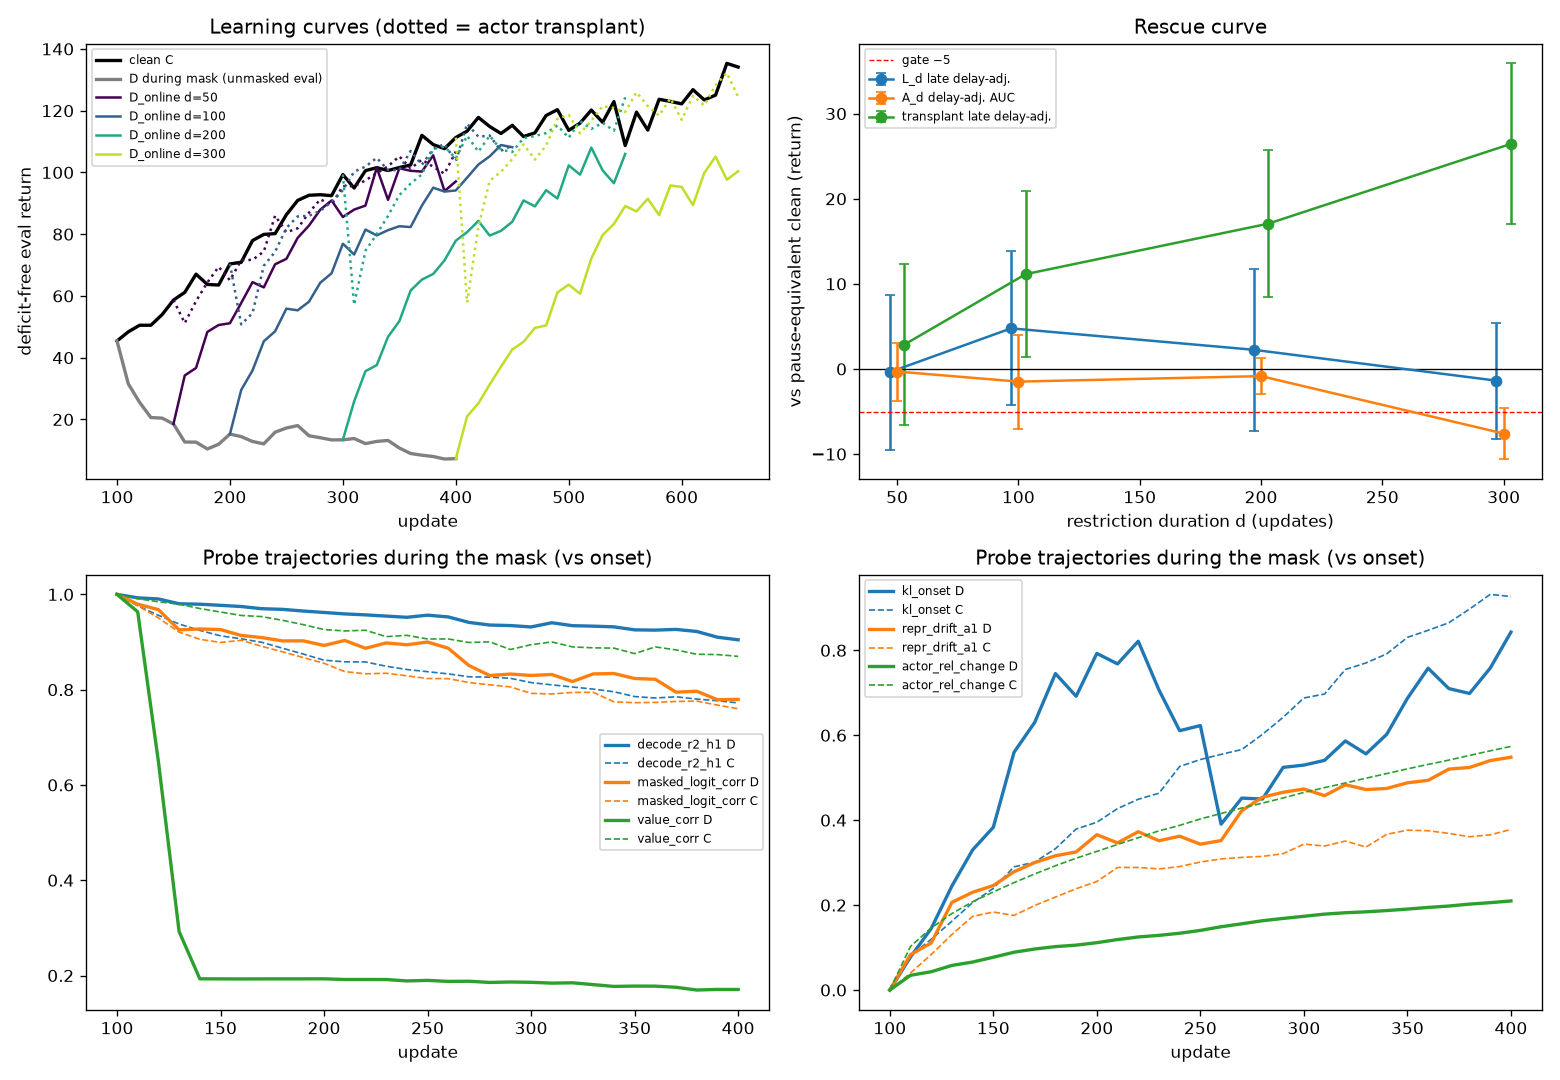
\includegraphics[width=\linewidth]{figures/p7_ponr_pilot.png}
\caption{Point-of-no-return pilot (PPO, movement restriction from $w_0=100$, durations $d\in\{50,100,200,300\}$, $n=4$). \textbf{Top left:} recovery curves (dotted: clean-actor transplant). \textbf{Top right:} delay-adjusted late deficit $L_d$, delay-adjusted AUC $A_d$ and transplant gain against $d$, with the pre-registered gate at $-5$. \textbf{Bottom:} probe trajectories during the restriction for D (solid) and C (dashed).}
\label{fig:ponr}
\end{figure}

\paragraph{Design.}
If damage is lost time, does it stay recoverable for arbitrarily long restrictions? All windows start at $w_0=100$ and are nested, so one restricted trajectory passes through the removal state for every duration $d$. Each removal is followed by a fixed budget of 250 recovery updates (2.05M steps).

The outcome $L_d$ is the delay-adjusted difference averaged over the last 40 updates of the budget; $A_d$ is the delay-adjusted AUC over the whole budget. A gate rule was committed before any data. Proceed to a confirmatory stage only if some $d$ gives mean $L_d\le-5$ with a 95\% interval below 0; stop otherwise.

\begin{table}[t]
\centering
\caption{Point-of-no-return pilot (PPO, $n=4$). $L_d$: delay-adjusted difference at the end of a 250-update budget; $A_d$: delay-adjusted AUC; ``raw'' compares with the clean run at the same absolute update. Negative = harm.}
\label{tab:ponr}
\small
\resizebox{\linewidth}{!}{%
\begin{tabular}{rcccccc}
\toprule
$d$ & removal eval D / C & $L_d$ & $A_d$ & raw AUC & transplant $-$ D & transplant $-$ C \\
\midrule
50  & 18.5 / 58.7  & $-0.4\ci{-9.5}{+8.7}$  & $-0.3\ci{-3.7}{+3.1}$ & $-11.5\sig$ & $+8.3\sig$  & $-3.2\ci{-6.8}{+0.5}$ \\
100 & 15.3 / 70.4  & $+4.8\ci{-4.3}{+13.8}$ & $-1.5\ci{-7.0}{+4.0}$ & $-22.6\sig$ & $+18.2\sig$ & $-4.4\ci{-9.5}{+0.7}$ \\
200 & 13.4 / 99.3  & $+2.3\ci{-7.2}{+11.7}$ & $-0.8\ci{-3.0}{+1.3}$ & $-33.9\sig$ & $+26.7\sig$ & $-7.1\ci{-14.2}{-0.1}\sig$ \\
300 & 7.3 / 111.3  & $-1.4\ci{-8.2}{+5.5}$  & $-7.6\ci{-10.6}{-4.6}\sig$ & $-48.8\sig$ & $+42.8\sig$ & $-6.1\ci{-14.2}{+2.1}$ \\
\bottomrule
\end{tabular}}
\end{table}

\paragraph{Result: STOP.}
No duration met the gate (Table~\ref{tab:ponr}), and the seed means of $L_d$ ($-0.4$, $+4.8$, $+2.3$, $-1.4$) do not decrease with $d$.
\begin{itemize}
\item Raw damage grows almost linearly with duration, from $-11.5$ to $-48.8$. Yet a restriction three times longer than the agent's entire pre-onset history leaves an agent back at the pause-equivalent level by the end of the budget.
\item The only cost beyond lost time is transient: slower early recovery at $d=300$ ($A_{300}=-7.6\ci{-10.6}{-4.6}$). It did not replicate in fresh seeds (see below).
\item The competent policy stays latent. At $d=300$, the onset policy's logits are linearly decodable from the damaged actor's features with $R^2=0.905$. That is higher than for the clean actor at the same update, which has moved past its onset policy.
\item The critic degrades within about 30 updates (value correlation with onset $\approx0.19$) and then stays flat.
\end{itemize}
With $n=4$ the $L_d$ intervals are about $\pm9$ wide, so an impairment near $-8$ at $d=300$ is not excluded. ``STOP'' means that none was detected.

\paragraph{Confirmatory test at $d=300$ (pre-registered, 8 fresh seeds).}
A null gate is not evidence of absence, so we pre-registered a confirmatory test at the longest duration: an equivalence test (TOST) against the gate's $\pm5$ margin on 8 fresh seeds (100--107). The decision rules were fixed in advance: \emph{equivalent} if both one-sided tests reject; \emph{persistent impairment} if the mean is $\le-5$ with an interval below 0; otherwise \emph{inconclusive}. The result is $L_{300}=+1.1\ci{-6.6}{+8.7}$ (TOST $p=0.13$): \textbf{inconclusive}. The point estimate is positive and the interval excludes impairments worse than $-6.6$, but one seed shows a large late deficit ($-17.6$), and the test lacks the power to establish equivalence within $\pm5$. Pooled with the pilot (descriptive only, $n=12$), $L_{300}=+0.2\ci{-4.7}{+5.1}$. The early cost had the same sign ($A_{300}=-4.6\ci{-12.3}{+3.0}$; pooled with the pilot $-5.6\ci{-10.4}{-0.8}$) but did not replicate in the later replication seeds (below). A clean-actor transplant again restores the agent to well above the pause reference ($+26.6\ci{+20.5}{+32.7}$).
We therefore claim only that no point of no return was \emph{detected} up to 2.46M restricted steps, and that persistent deficits larger than about 7 return points are excluded at $d=300$. We do not claim that the deficit is zero.

\paragraph{Independent replication at $d=300$ (pre-registered; incomplete, descriptive).}
In a second reviewer-response round we pre-registered an independent replication with 32 fresh seeds (300--331). It had about 84\% power to declare equivalence within $\pm5$ if the true deficit were 0, and it pre-registered a powered test of the removal-time predictors (below). Two sandbox restarts cost a third of the compute budget, and only 16 seeds (300--315) were completed. As pre-registered for this case, we report them descriptively, without a decision: $L_{300}=+6.0\ci{+1.9}{+10.2}\sig$ and $A_{300}=+1.3\ci{-0.7}{+3.3}$. Pooled with the Phase~8 seeds (descriptive, $n=24$): $L_{300}=+4.4\ci{+0.8}{+7.9}\sig$ and $A_{300}=-0.7\ci{-3.4}{+2.1}$.
In the replication seeds, harm worse than $-5$ is rejected (one-sided $p<10^{-4}$). Equivalence within $\pm5$ would still fail, because a benefit above $+5$ cannot be excluded. The pooled interval lies above zero, so the restricted agents end slightly \emph{ahead} of a paused control. This is consistent with the small amount of learning that happens under the restriction, which the pause baseline does not credit (Section~\ref{sec:estimands}). Only the 4-seed pilot ($[-8.2,+5.5]$) left room for a deficit of several points. The early-recovery cost seen in the pilot ($A_{300}=-7.6\sig$) and, in direction, in the Phase~8 seeds did not appear in the replication seeds ($A_{300}=+1.3\ci{-0.7}{+3.3}$), so we no longer report it as a finding. These pooled statements are descriptive. We do not claim that a point of no return is absent at longer restrictions or in other settings, only that none was detected here.

\paragraph{Removal-time predictors (pre-specified): none found in our samples.}
We then asked whether a measurement taken at removal predicts \emph{which} agents recover slowly, beyond duration. Before computing any metric we fixed four candidates and pass criteria R0--R3. The candidates were:
\begin{itemize}
\item policy divergence from the clean fork (KL);
\item representation divergence ($1-$CKA; \citealp{kornblith2019cka});
\item relative change of the restricted actions' probabilities in relevant states;
\item critic error against the clean critic.
\end{itemize}
The criteria were: R0, measurement reliability; R1, pooled rank correlation with recovery cost; R2, rank correlation within duration; R3, leave-one-seed-out predictive gain over a duration-only model.

All four were reliable measurements (R0: 0.87 to 0.99) and correlated with recovery cost when pooled across durations. None passed: within-duration correlations were $+0.05$, $-0.11$, $+0.13$ and $-0.35$, and every candidate \emph{reduced} out-of-fold accuracy (gains of $-25\%$, $-8\%$, $-8\%$ and $-83\%$). The pooled associations come entirely from the shared trend with duration. One pre-specified secondary analysis, re-computing the metrics early in recovery, was not run; we disclose this as a deviation (Appendix~\ref{app:prov}).

In the replication seeds at $d=300$ (descriptive, $n=16$; Table~\ref{tab:predictors}), the four predictors' rank correlations with the recovery cost $A_{300}$ were $-0.24$ (KL), $-0.13$ ($1-$CKA), $-0.15$ (restricted-action change) and $+0.18$ (critic error). The pre-registered direction was negative: more divergence, slower recovery. Three are in that direction, but all are weak, every interval includes zero, and every predictor \emph{reduced} leave-one-out accuracy (gains $-8\%$ to $-21\%$).

\begin{table}[t]
\centering
\caption{Removal-time predictors vs.\ recovery cost $A_{300}$ in the replication seeds (descriptive; the pre-registered $n=32$ test was not completed). $\rho$: Spearman correlation; 95\% CI by Fisher $z$ with the Bonett--Wright standard error. The pre-registered direction is $\rho<0$. Split-half: predictor reliability across halves of the evaluation-state bank. LOO gain: leave-one-out $R^2$ gain of a one-predictor linear model over the mean. Source: \url{p9_ponr_predictors-analysis.md}.}
\label{tab:predictors}
\small
\begin{tabular}{lcccc}
\toprule
predictor & split-half & $\rho$ with $A_{300}$ & 95\% CI for $\rho$ & LOO gain \\
\midrule
policy divergence (KL) & $0.87$ & $-0.24$ & $[-0.66,+0.30]$ & $-18\%$ \\
representation divergence ($1-$CKA) & $0.71$ & $-0.13$ & $[-0.59,+0.39]$ & $-21\%$ \\
restricted-action change & $0.96$ & $-0.15$ & $[-0.60,+0.38]$ & $-14\%$ \\
critic error & $0.65$ & $+0.18$ & $[-0.35,+0.62]$ & $-8\%$ \\
\bottomrule
\end{tabular}
\end{table}

\paragraph{``No predictor found'' is not ``unpredictable''.} We keep two claims apart.
\begin{itemize}
\item \emph{What we found.} In the pilot (4 seeds per duration), no pre-specified measurement passed the pre-specified criteria. In the replication seeds, no measurement showed a reliable association in the pre-registered direction. This is a statement about our samples.
\item \emph{What we do not claim.} We do not claim that these measurements cannot predict recovery. Three facts argue against that reading. (i) Both sides of the relation are measured reliably: the predictors' split-half reliabilities are high, and the outcome $A_{300}$ has a split-half reliability of 0.95 in the Phase~8 seeds and 0.78 in the replication seeds. Measurement noise therefore does not cap predictability. (ii) The confidence intervals for $\rho$ still include moderate negative correlations, down to $-0.59$ to $-0.66$ for the three divergence measures. (iii) Detecting $\rho=-0.4$ with 80\% power under Holm correction across four predictors requires about 59 agents at a single duration. The pre-registered 32 were chosen for $\rho\approx-0.5$, and we completed 16.
\end{itemize}
Recovery cost may well be predictable from removal-time measurements, with these or other metrics. Our data only exclude very strong single-predictor relations (Table~\ref{tab:predictors}).

What does replicate is that early and late recovery costs are unrelated ($\rho=-0.01$ in the pilot, $-0.05$ in the Phase~8 seeds): agents that recover slowly at first do not end up worse. The outcome-reliability analysis is post-hoc. Its pilot estimate (Spearman--Brown 0.30, from 4-seed rankings at short durations) was contradicted by the Phase~8 seeds (0.95 at $d=300$), and we withdrew a ``predictor ceiling'' interpretation from an earlier draft.

%=====================================================================
\section{Does the localization generalize? (pre-registered)}\label{sec:general}
%=====================================================================

All results so far come from one game, one deficit family and one network size. Before running anything, we pre-registered three generalization tests of the PPO $2^3$ surgery, each with 8 seeds and the same analysis and fixed criterion. The localization \emph{replicates} if total damage has an interval below 0, the actor main effect has an interval below 0, and the actor has the largest Shapley share. If total damage is not detectably negative, the verdict is ``no damage to localize'' rather than a failure. The three tests were:
\begin{itemize}
\item a second game (Asterix-MinAtar, no left/right, onset at the meaning-matched update 390 located from a long control);
\item a different deficit family (reward sign flip with probability 1 during the late window, SpaceInvaders);
\item a wider network ($2\times256$ actor and critic, movement restriction, SpaceInvaders).
\end{itemize}

\begin{table}[t]
\centering
\caption{Pre-registered generalization of the PPO state surgery (late window, recovery AUC; paired 95\% $t$-intervals). ``Gap at removal'' = damaged $-$ clean at removal. Delay-adjusted AUC = damaged $-$ clean shifted by the window length (requires evaluation during the window; not run for the original seeds). Shapley share = actor's share of total damage (ratio of means). Sources: \url{p8_ppo_surgery_n12-analysis.md}, \url{p8_asterix_surgery-analysis.md}, \url{p8_rflip_surgery-analysis.md}, \url{p8_h256_surgery-analysis.md}, \url{p9_asterix_rflip_surgery-analysis.md}. The Asterix reward-flip row was pre-registered in Phase 9 with 8 seeds and run with 4 (deviation).}
\label{tab:general}
\small
\resizebox{\linewidth}{!}{%
\begin{tabular}{lcccccccl}
\toprule
setting & $n$ & gap at removal & total damage & delay-adj.\ AUC & actor & critic & optimizer & actor share; verdict \\
\midrule
SpaceInvaders, movement, $2\times128$ & 12 & $-37.0\ci{-45.1}{-28.9}\sig$ & $-15.1\ci{-17.2}{-13.0}\sig$ & -- & $-13.7\sig$ & $-1.9\sig$ & $+0.2$ & 90\%; replicates \\
Asterix, movement, $2\times128$ & 8 & $-1.0\ci{-1.5}{-0.5}\sig$ & $-0.1\ci{-0.5}{+0.4}$ & $+0.5\ci{+0.0}{+1.0}\sig$ & $-0.2$ & $-0.0$ & $+0.0$ & n/a; no damage to localize \\
SpaceInvaders, reward flip, $2\times128$ & 8 & $-58.2\ci{-66.4}{-50.1}\sig$ & $-32.3\ci{-40.7}{-23.9}\sig$ & $-18.6\ci{-27.2}{-9.9}\sig$ & $-32.8\sig$ & $+1.2$ & $-1.9$ & 100\%; replicates \\
Asterix, reward flip, $2\times128$ (Phase 9) & 4 & $-4.2\ci{-6.0}{-2.4}\sig$ & $-2.4\ci{-3.6}{-1.2}\sig$ & $-1.8\ci{-2.6}{-1.0}\sig$ & $-2.2\sig$ & $-0.1$ & $+0.0$ & 93\%; replicates \\
SpaceInvaders, movement, $2\times256$ & 8 & $-49.9\ci{-56.9}{-43.0}\sig$ & $-19.7\ci{-23.7}{-15.6}\sig$ & $-5.1\ci{-8.3}{-1.8}\sig$ & $-15.7\sig$ & $-2.5\sig$ & $-0.4$ & 82\%; replicates \\
\bottomrule
\end{tabular}}
\end{table}

\paragraph{Second game.} On Asterix the late movement restriction again caused unlearning during the window, but only a little: $-1.0\ci{-1.6}{-0.3}$, about 18\% of the clean agent's competence. It was followed by complete recovery. The restricted agent ends slightly \emph{ahead} of a paused control (delay-adjusted $+0.5\ci{+0.0}{+1.0}$), and there is no persistent damage to localize (total $-0.1\ci{-0.5}{+0.4}$). The short-lived deficit sits in the actor ($-1.0\ci{-1.3}{-0.6}$ at $+10$ updates) and has gone by $+50$.

\paragraph{Different deficit.} Flipping the reward sign is a far harsher deficit. The agent learns to avoid reward, and its unmasked return drops to exactly 0 at removal. Unlike the action restriction, it causes damage beyond lost time within the 150-update budget (delay-adjusted AUC $-18.6\ci{-27.2}{-9.9}$). The carrier is the same: the actor's Shapley value equals the total damage ($-32.4$ of $-32.3$), neither critic nor optimizer state contributes detectably, and a clean-actor transplant restores the damaged agent to the clean agent's level ($-0.4\ci{-3.4}{+2.5}$ vs.\ clean).

\paragraph{Wider network.} Doubling the width of both networks ($2\times256$) leaves the picture unchanged. The late movement restriction causes unlearning ($-28.7\ci{-36.4}{-21.0}$) and a recovery deficit of $-19.7$ AUC. The actor carries 82\% of it (Shapley $-16.1\ci{-18.0}{-14.1}$), the critic again adds a small, early contribution ($-2.9\ci{-5.4}{-0.4}$, 15\%; $-10.1$ at $+10$ updates, $+1.0$ at $+150$), and Adam state is equivalent to zero within $\pm3$ (TOST $p=0.013$). A clean-actor transplant rescues $+15.7\ci{+11.7}{+19.7}$.

\paragraph{Why Asterix showed no lasting damage under the movement restriction.}
Asterix is counterevidence to any claim that late deficits \emph{always} cause lasting damage, and we make no such claim. Two features of that setting predicted a null under the lost-competence account of Section~\ref{sec:timing}.
\begin{itemize}
\item \emph{Little competence was lost.} Removing left and right in Asterix still leaves up and down movement, so the restricted policy kept most of its competence (gap at removal 18\%, against 63--100\% in the SpaceInvaders settings).
\item \emph{There was no progress to lose.} The clean agent made no progress during the window (5.36 to 5.41), so the restricted agent had no lost progress to make up. In SpaceInvaders the clean agent improved by 28--45\% in the same window.
\end{itemize}
To test whether the null was specific to the game or to the deficit, we pre-registered the same surgery on Asterix with the harsher reward-flip deficit (Phase 9; run with 4 seeds after compute loss). The flip removed 70\% of competence by removal ($-4.2\ci{-6.0}{-2.4}$), while the clean agent again made no progress. This time there was lasting damage beyond lost time: delay-adjusted AUC $-1.8\ci{-2.6}{-1.0}$, still $-1.2\ci{-2.2}{-0.1}$ at the end of the 200-update budget. The total was $-2.4\ci{-3.6}{-1.2}$, and the localization criterion was met. The actor's Shapley share is 93\% (4/4 seeds), critic and optimizer state are each equivalent to zero within $\pm3$ (TOST $p\le10^{-4}$), and a clean actor restores the clean agent's level ($+0.1\ci{-0.9}{+1.0}$ vs.\ clean). The Asterix null was therefore a property of the mild deficit, not of the game.

\emph{Post-hoc, across settings} (Table~\ref{tab:gap}; descriptive, five settings): total damage grows with the fraction of competence lost at removal. It is $-2\%$ of the clean agent's competence at a gap of 18\%, $-26$ to $-40\%$ at 63--73\%, and $-55\%$ at 100\%. Damage beyond lost time appears in the settings with the largest gaps. The pattern is consistent with a simple account: lasting damage requires that the deficit destroys more competence than can be relearned within the budget, plus whatever progress the clean agent makes meanwhile. Whenever damage of either kind exists, the actor carries most of it.

\begin{table}[t]
\centering
\caption{Post-hoc (descriptive): competence lost at removal vs.\ damage across the PPO surgery settings. Relative quantities are divided by the clean agent's competence at removal $C(w_1)$. Clean progress: $C(w_1)-C(w_0)$ during the window. $^\ast$ SpaceInvaders $2\times128$ has no evaluation during the window for its 12 surgery seeds; $C(w_0)$ and $C(w_1)$ are from the Phase~2 seeds 0--3. Source: \url{p9_gap_vs_damage-posthoc.md}.}
\label{tab:gap}
\small
\resizebox{\linewidth}{!}{%
\begin{tabular}{lccccccc}
\toprule
setting & $n$ & clean progress & gap at removal & relative gap & total damage & relative total & delay-adj.\ AUC \\
\midrule
Asterix, movement & 8 & $+1\%$ & $-1.0\sig$ & $18\%$ & $-0.1\ci{-0.5}{+0.4}$ & $-2\%$ & $+0.5\ci{+0.0}{+1.0}\sig$ \\
SpaceInvaders, movement, $2\times128^\ast$ & 12 & $+29\%$ & $-37.0\sig$ & $63\%$ & $-15.1\sig$ & $-26\%$ & -- \\
Asterix, reward flip & 4 & $0\%$ & $-4.2\sig$ & $70\%$ & $-2.4\sig$ & $-40\%$ & $-1.8\ci{-2.6}{-1.0}\sig$ \\
SpaceInvaders, movement, $2\times256$ & 8 & $+45\%$ & $-49.9\sig$ & $73\%$ & $-19.7\sig$ & $-29\%$ & $-5.1\ci{-8.3}{-1.8}\sig$ \\
SpaceInvaders, reward flip & 8 & $+28\%$ & $-58.2\sig$ & $100\%$ & $-32.3\sig$ & $-55\%$ & $-18.6\ci{-27.2}{-9.9}\sig$ \\
\bottomrule
\end{tabular}}
\end{table}

In the four settings with damage to localize, the actor carries most of it (82--100\%). In both SpaceInvaders movement settings the critic adds a small, significant, early share (12\%, 15\%); in the two reward-flip settings it was not detected.

%=====================================================================
\section{Discussion}
%=====================================================================

\paragraph{Lost competence, not lost plasticity.}
Across three learners, the evidence is consistent:
\begin{itemize}
\item early deficits cost time;
\item late deficits cause unlearning that is relearned, and from equal competence restricted agents relearn faster than clean agents first learned (a savings effect confirmed on fresh seeds, Table~\ref{tab:estimands});
\item the damaged network retains a decodable copy of the competent policy and outperforms a fresh one;
\item what persists is the progress the clean agent made in the meantime, stored in the function approximator.
\end{itemize}
In PPO the main carrier is the actor's parameters (Shapley share 82--100\% across settings). The critic is a minor carrier: significant at $n=12$ (12\%) and with the wider network (15\%), concentrated in the first updates of recovery, and not detected under the reward flip. Adam moments are equivalent to zero within $\pm3$, which complements optimizer-state accounts in other settings \citep{dohare2023collapse,xu2026optimizer}. In PQN-R the carrier is the Q-network's parameters; RAdam state matters only for a brief transient. A large buffer extends the period during which restricted data shape the network, but its effect outlasts the data, so it mediates the damage rather than storing it.

\paragraph{Relation to the primacy bias and resets.}
\citet{nikishin2022primacy} found that resetting parts of an agent while keeping its buffer cures early overfitting. In our setting resets are harmful: an actor reset costs $-27.2$. The difference is informative. Primacy-bias damage is a network fitted to stale early data whose capacity to fit new data is impaired. Ours is a network that has drifted away from a competence it can quickly regain. A reset discards both the damage and the retained competence, and the second matters more.

\paragraph{Practical implications.}
For agents subject to temporary action constraints or similar deficits:
\begin{enumerate}[label=(\roman*)]
\item do not reset after the deficit;
\item protecting the policy during the deficit (freezing, KL anchoring) preserves evaluation performance during the deficit but did not detectably speed recovery (gains above $+5.7$ and $+1.7$ AUC are excluded, $n=4$);
\item in replay agents, refreshing the buffer with fresh, competent data helps modestly, and keeping the replacement resident longer matters about as much as which data is removed;
\item when a clean policy from a parallel run is available, transplanting it is effective, as is briefly training on its data with importance weighting, which acts as off-policy distillation; the same data without importance weighting is harmful.
\end{enumerate}

\paragraph{Limitations.}
\begin{itemize}
\item \textbf{Scope.} The main environment is SpaceInvaders-MinAtar in gymnax, whose dynamics differ from MinAtar. Generalization was tested on one more game, one more deficit family and one wider MLP (Section~\ref{sec:general}). On Asterix the movement restriction caused no persistent damage. The carrier claim on Asterix rests on the reward-flip test, which has only 4 seeds. Lasting damage is not universal: it was absent when the deficit removed little competence. Larger convolutional agents, high replay ratios \citep{schwarzer2023bbf}, continuous control and other deficits may behave differently.
\item \textbf{Seeds.} The PPO surgery now has 12 seeds and the generalization tests 8. Several secondary results (drift suppression, PQN early/late recovery, fire restriction) still rest on 4 seeds. Appendix Table~\ref{tab:power} gives their minimum detectable effects, and we phrase them as bounds.
\item \textbf{Point of no return and predictors.} The confirmatory test was inconclusive, and the powered replication was not completed. Persistent deficits of a few return points at long restrictions are not excluded. The predictor results are bounds from small samples: moderate correlations with recovery cost remain compatible with our data.
\item \textbf{Data versus update rule in PPO.} The ratio-neutral swap removes importance weighting, but it applies on-policy updates to off-policy actions. No PPO arm cleanly isolates data content from the update rule.
\item \textbf{Counterfactual baseline.} Numerical ``damage'' depends on the counterfactual. We fix one estimand per question (Section~\ref{sec:estimands}) and test both primaries confirmatorily only for PPO's late movement restriction. For the other learners the comparison is post-hoc and rests on 4 seeds. The pause baseline assumes that a restricted update is worth nothing, whereas some learning does happen under the restriction (early windows, Table~\ref{tab:ppo_recovery}). It can therefore favour the restricted agent slightly. The carrier analysis compares components at the same update and does not depend on this choice.
\item \textbf{Marginal equivalence.} The rung-4 equivalence result clears its margin only narrowly. We claim only that identity effects of $\geq1$ AUC point are excluded.
\item \textbf{Exploratory early phases.} The PPO and PQN phases before the purge study preceded our pre-registration practice. Their central PPO claim has since been replicated under pre-registration.
\end{itemize}

%=====================================================================
\section{Conclusion}
%=====================================================================
In our settings, temporary action restrictions did not open a detectable early critical period. Imposed after competence has emerged, they cause unlearning that is relearned, and the residual cost is lost progress stored in the function approximator's parameters. In PPO it is mostly the actor (82--100\% of the damage, also under a reward-flip deficit, with a wider network and on a second game), plus a small, significant but transient critic share (12--15\% under the movement restriction). In PQN-R it is the Q-network. Replay data mediate this damage while they are consumed but do not store it, and the apparent data-identity effect largely disappears once slot age and residence are matched. Within 2.46M steps of restriction we detect no point of no return (large persistent deficits are excluded; small ones are not). Four pre-specified removal-time measurements did not predict slow recovery in our samples, a bound on their predictive strength rather than evidence that recovery is unpredictable. We hope the protocol (matched forks, unmasked common-random-number evaluation, delay-adjusted recovery and factorial state surgery) is useful for locating the carriers of other training pathologies in RL.

\subsubsection*{Broader impact statement}
This is basic research on training dynamics in small simulated environments. We do not foresee direct negative societal impacts. Understanding how agents recover from temporary constraints may inform the safe deployment of RL systems in which actions are sometimes disabled.

\subsubsection*{Reproducibility statement}
All code, configurations, run manifests (with commit hashes and package versions), per-seed results, analysis scripts and a chronological experiment log with every pre-registration are available at \repo. Pinned versions: jax 0.11.2, flax 0.12.10, optax 0.2.8, gymnax 0.0.9, numpy 2.5.4. Runs are deterministic on CPU given the seed. Each experiment fits on a 2-core CPU without a GPU; for example, the PPO recovery test took 1{,}883\,s and the point-of-no-return pilot 2{,}683\,s. Appendix~\ref{app:prov} maps every table to its source files.

\bibliography{refs}
\bibliographystyle{tmlr}

\newpage
\appendix

%=====================================================================
\section{Hyperparameters}\label{app:hparams}
%=====================================================================

\begin{table}[h]
\centering
\caption{Agent hyperparameters (SpaceInvaders-MinAtar, flattened $10\times10\times6$ observations).}
\label{tab:hparams}
\small
\resizebox{\linewidth}{!}{%
\begin{tabular}{lll}
\toprule
 & PPO & PQN / PQN-R \\
\midrule
network & separate actor/critic MLP $2\times128$, ReLU & Q-MLP $2\times128$, LayerNorm, ReLU \\
initialization & orthogonal ($\sqrt2$; heads 0.01 / 1.0) & Flax default \\
environments $\times$ steps & $64\times128$ (8{,}192 per update) & $128\times32$ (4{,}096 per update) \\
optimization & 4 epochs $\times$ 8 minibatches & 2 epochs $\times$ 32 minibatches \\
optimizer, LR & Adam, $5\cdot10^{-4}$ constant & RAdam, $5\cdot10^{-4}$ constant \\
gradient clip (global norm) & 0.5 & 10 \\
discount, trace & $\gamma=0.99$, GAE $\lambda=0.95$ & $\gamma=0.99$, Q($\lambda{=}0.65$) (PQN) \\
loss terms & clip 0.2, entropy 0.01, value 0.5 & $\tfrac12$ squared TD error \\
exploration & stochastic policy & $\epsilon$: 1 $\to$ 0.05 over 1M steps \\
replay (PQN-R) & -- & FIFO 100k or 1M, batch 128, 1-step, replay ratio 2, no target net \\
early / late window & updates $[0,50)$ / $[100,150)$ & updates $[0,100)$ / $[250,350)$ \\
window length & 409{,}600 env steps & 409{,}600 env steps \\
evaluation & every 10 updates, 64 episodes, stochastic & every 10 updates, 64 episodes, $\epsilon=0.05$ \\
\bottomrule
\end{tabular}}
\end{table}

%=====================================================================
\section{Provenance, pre-registration timeline and deviations}\label{app:prov}
%=====================================================================

Every number in the main text comes verbatim from an analysis file in \texttt{results/summary/} of the repository, after the sign conversion stated in Section~\ref{sec:protocol}. Each analysis reads only committed run summaries, and each run manifest records its commit hash, whether the working tree was clean, configuration and package versions.

\begin{table}[h]
\centering
\caption{Sources of the reported results.}
\footnotesize
\begin{tabular}{p{3.0cm}p{7.6cm}p{4.0cm}}
\toprule
result & analysis file (\url{results/summary/}) & design status \\
\midrule
Table~\ref{tab:ppo_recovery} & \url{p2_recovery_all-analysis.md} & exploratory \\
Table~\ref{tab:pqn_recovery} & \url{p5_recovery_move-analysis.md} & exploratory; metric fixed before analysis \\
Table~\ref{tab:ppo_surgery} & \url{20261011-p3-surgery-move-late-analysis.md}, \url{20261011-p4-phase4-move-late-...-analysis.md}, \url{20261011-p4-phase4-fire-late-...-analysis.md} & exploratory \\
Table~\ref{tab:pqnr} & \url{p6_surgery_pqnr_n12-analysis.md}, \url{p6_surgery_pqnr1m_n8-analysis.md}, \url{*-phases.md} & assignment rule pre-specified \\
Table~\ref{tab:ladder}, rung 1 & \url{p6_purge-analysis.md}, \url{p6_purge-posthoc.md} & pre-registered (864697e) \\
rung 2 & \url{p6b_targeted-analysis.md} & pre-registered; runs at 250cec4 \\
rung 3 & \url{p6c_2x2-analysis.md}, \url{p6c_2x2-factorial-posthoc.md} & pre-registered; runs at 2559f2e; ANOVA post-hoc \\
rung 4 & \url{p6d_idswap-analysis.md} & pre-registered (a873dc0), $n$ and SESOI fixed \\
Table~\ref{tab:ponr} & \url{p7_ponr_pilot-analysis.md} & gate pre-registered (ba1802f) \\
predictors & \url{p7b_predictors-analysis.md} & pre-specified (aabd1ae), script 39c3049 \\
Table~\ref{tab:ppo_surgery} ($n=12$), data arms & \url{p8_ppo_surgery_n12-analysis.md} & pre-registered (8c62fe0); seeds 0--3 exploratory \\
PQN-R parameters vs.\ optimizer & \url{p8_pqnr_split-analysis.md} & pre-registered (8c62fe0) \\
confirmatory $d=300$ & \url{p8_ponr_confirm-analysis.md} & pre-registered (8c62fe0) \\
Table~\ref{tab:general} & \url{p8_asterix_surgery-analysis.md}, \url{p8_rflip_surgery-analysis.md}, \url{p8_h256_surgery-analysis.md} & pre-registered (8c62fe0) \\
Table~\ref{tab:estimands} & \url{p9_estimands-analysis.md} & pre-registered (63a8f1d) \\
replication $d=300$, Table~\ref{tab:predictors} & \url{p9_ponr_predictors-analysis.md} & pre-registered (63a8f1d); incomplete, descriptive \\
Asterix reward flip & \url{p9_asterix_rflip_surgery-analysis.md} & pre-registered (63a8f1d); $n=4$ (deviation) \\
Table~\ref{tab:gap} & \url{p9_gap_vs_damage-posthoc.md} & post-hoc \\
Tables~\ref{tab:power}, \ref{tab:baselines}; rung-4 sensitivity & \url{p8_power-posthoc.md}, \url{p8_alt_baselines-posthoc.md}, \url{p8_6d_sensitivity-posthoc.md} & post-hoc \\
\bottomrule
\end{tabular}
\end{table}

\paragraph{Deviations and corrections.}
\begin{enumerate}[label=(\arabic*)]
\item Early PPO analyses used percentile bootstrap intervals over 4 seeds. These were replaced by paired $t$-intervals. This reversed one conclusion: the PPO delay-adjusted residual at $+250$ updates changed from significant to $+2.0\ci{-0.1}{+4.1}$.
\item The purge study's E arm (purge on the clean network) was added by us as a secondary arm before data collection. The B$-$E contrast was computed post-hoc.
\item In Phase 6c, the factorial ANOVA was requested after the results and is labelled post-hoc. Only its interaction term had been pre-registered, as a descriptive secondary.
\item In Phase 7b, secondary item 1 (the predictor metrics at $+10/+20/+30$ updates of recovery) was not run. Its outcome variables have the same low reliability as the primary ones, so it could not change the verdict. The run is deterministic and can be reproduced.
\item The outcome-reliability analysis of Section~\ref{sec:ponr} is post-hoc. Its pilot estimate (0.30) was contradicted by the Phase~8 seeds (0.95 at $d=300$), and we withdrew the ``predictor ceiling'' interpretation from an earlier draft.
\item Phase 8 (reviewer response). All runs, contrasts, margins and decision rules were committed before data (8c62fe0). The analysis scripts were written during the runs and implement only those contrasts; the baseline comparison, the rung-4 sensitivity analysis and the minimum-detectable-effect table are post-hoc. Twice the run queue stopped because the paper source or an untracked script made the working tree dirty, which the provenance guard refuses. No run was affected, and the queue resumed after a commit. The reproduction check against the Phase 2 reference is valid only for seeds 0--3, since the reference contains no other seeds. Seeds 0--3 matched exactly, and the Phase 8 DDD cells reproduced the earlier arms bit for bit.
\item Phase 9 (second reviewer response). Estimands, runs, margins, tests and decision rules were committed before data (63a8f1d), together with analysis scripts validated on earlier data only. E1 ran as planned. Two sandbox restarts cost about a third of the 6\,h budget. With the authors' decision, recorded before any E3 outcome was analysed, the Asterix reward-flip test was cut to 4 seeds and the point-of-no-return replication stopped at 16 of 32 seeds. Per its pre-registered fallback, the replication is reported descriptively without a decision. All deviations are logged with timestamps (commits 4a02dd2 and later).
\item Two conclusions of the earlier draft changed with more seeds or better controls: the PPO critic is not uninvolved (a small transient effect at $n=12$), and the PPO data-swap benefit is not a data-content effect (it disappears without importance weighting).
\end{enumerate}

%=====================================================================
\section{Additional results}
%=====================================================================

\begin{figure}[h]
\centering
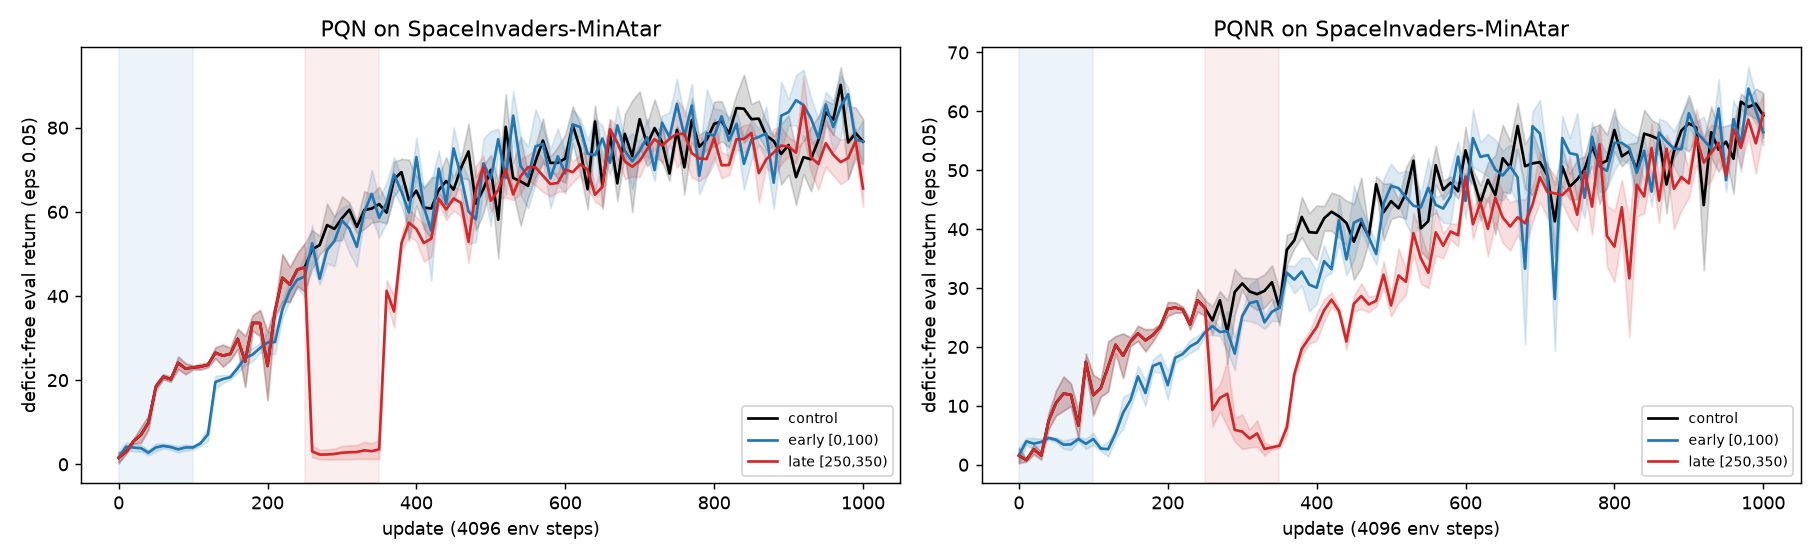
\includegraphics[width=\linewidth]{figures/p5_recovery_move.png}
\caption{PQN and PQN-R recovery after early and late movement restrictions ($n=4$).}
\label{fig:pqn_recovery}
\end{figure}

\begin{figure}[h]
\centering
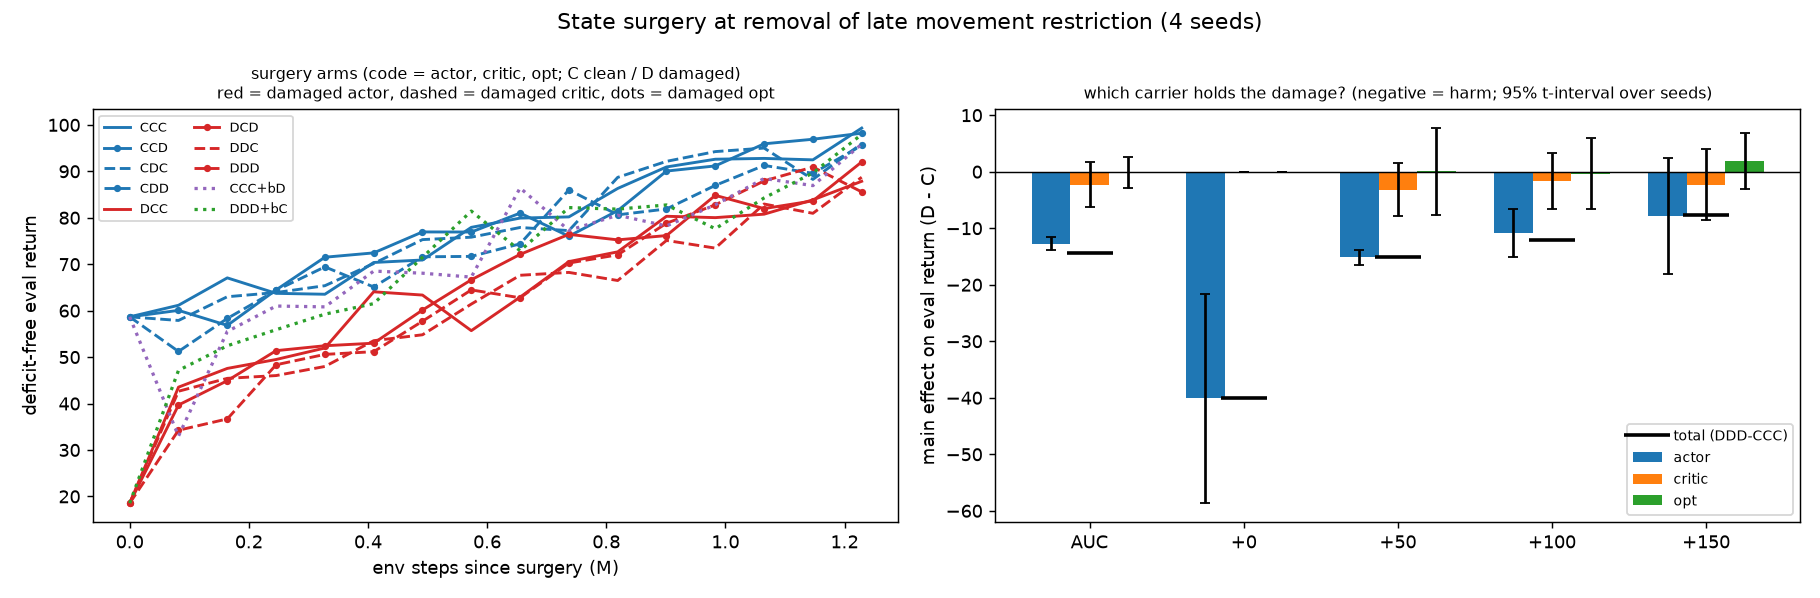
\includegraphics[width=\linewidth]{figures/surgery_move_late.png}
\caption{PPO $2^3$ actor $\times$ critic $\times$ optimizer surgery after the late movement restriction ($n=4$).}
\label{fig:ppo_surgery}
\end{figure}

\begin{figure}[h]
\centering
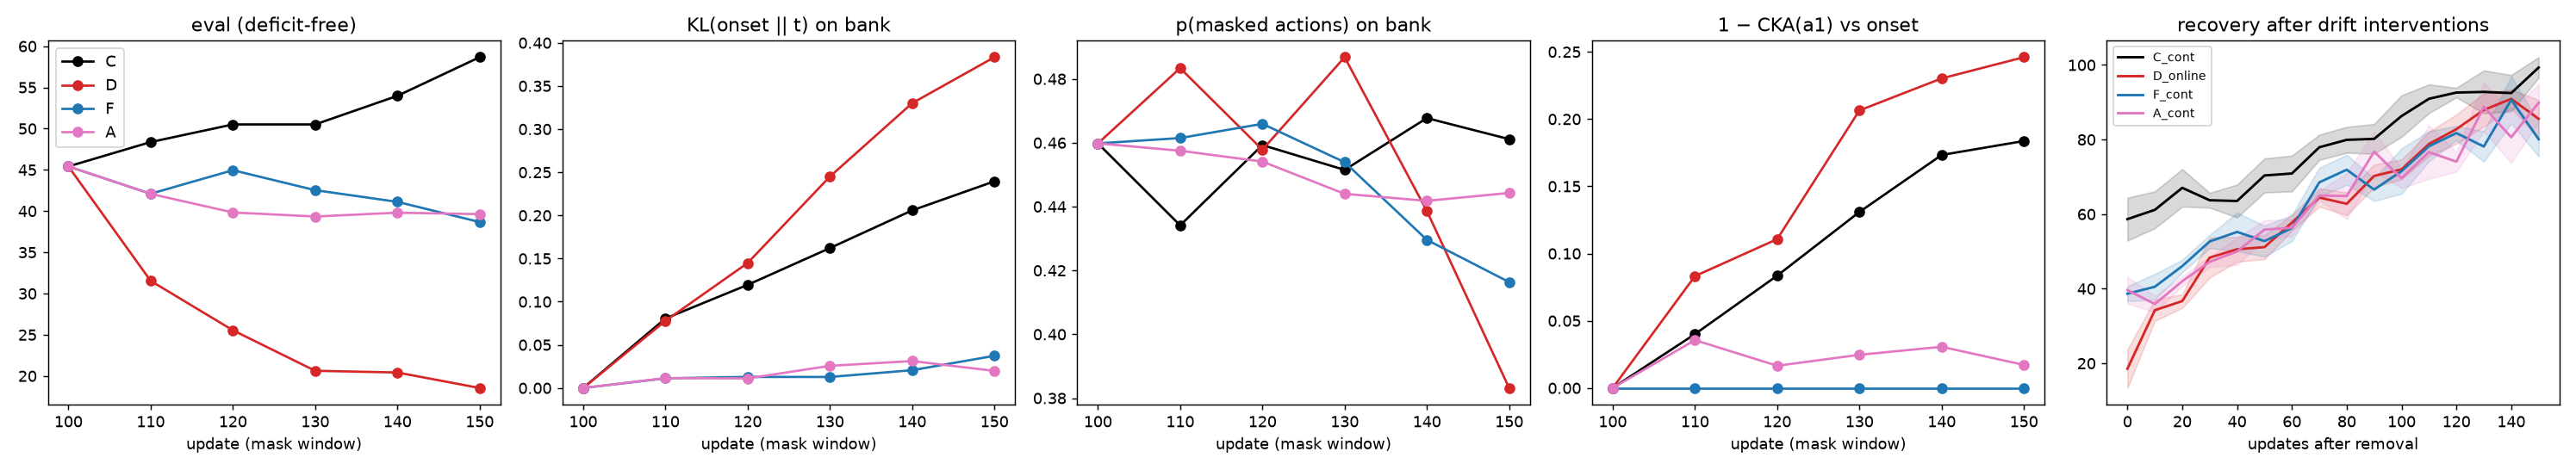
\includegraphics[width=\linewidth]{figures/phase4_move_late_drift.png}
\caption{PPO drift suppression during the restriction. F: actor hidden layers frozen; A: KL anchor to the onset policy. Both raise evaluation at removal but leave recovery AUC unchanged.}
\label{fig:drift}
\end{figure}

\begin{table}[h]
\centering
\caption{PPO drift-suppression arms at removal and during recovery ($n=4$; paired differences vs.\ the unprotected restricted agent D unless stated).}
\small
\begin{tabular}{lcccc}
\toprule
arm & KL from onset & 1$-$CKA (layer a1) & eval at removal & recovery AUC \\
\midrule
C (clean) & 0.239 & 0.184 & 58.7 & 79.3 \\
D (restricted) & 0.383 & 0.246 & 18.5 & 65.0 \\
F (frozen torso) & 0.037 & 0.000 & 38.7 & 66.1 \\
A (KL anchor) & 0.020 & 0.017 & 39.6 & 64.9 \\
\midrule
F $-$ D & & & $+20.1\ci{+8.2}{+32.0}\sig$ & $+1.1\ci{-3.4}{+5.7}$ \\
A $-$ D & & & $+21.1\ci{+13.1}{+29.0}\sig$ & $-0.0\ci{-1.8}{+1.7}$ \\
F $-$ C & & & $-20.0\ci{-33.5}{-6.5}\sig$ & $-13.2\ci{-20.0}{-6.4}\sig$ \\
A $-$ C & & & $-19.0\ci{-36.0}{-2.1}\sig$ & $-14.4\ci{-18.5}{-10.3}\sig$ \\
\bottomrule
\end{tabular}
\end{table}

\begin{table}[h]
\centering
\caption{Post-hoc: minimum detectable effects (MDE, 80\% power, two-sided $\alpha=0.05$, paired $t$) of the small-$n$ null results, derived from the reported intervals. ``Excluded beyond'' is the interval's lower bound. Rows marked $^\ddagger$ were superseded by pre-registered larger-$n$ tests. Source: \url{p8_power-posthoc.md}.}
\label{tab:power}
\small
\begin{tabular}{lcccc}
\toprule
contrast & $n$ & estimate & MDE & harm excluded beyond \\
\midrule
PPO move late, delay-adjusted at $+250$ & 4 & $+2.0\ci{-0.1}{+4.1}$ & 2.7 & $-0.1$ \\
PPO fire late, delay-adjusted at $+250$ & 4 & $+2.4\ci{-3.6}{+8.3}$ & 7.8 & $-3.6$ \\
PQN late, delay-adjusted AUC & 4 & $-1.4\ci{-3.5}{+0.7}$ & 2.7 & $-3.5$ \\
PQN-R late, delay-adjusted at $+650$ & 4 & $-0.2\ci{-7.7}{+7.3}$ & 9.8 & $-7.7$ \\
drift suppression F $-$ D, AUC & 4 & $+1.1\ci{-3.4}{+5.7}$ & 5.9 & $-3.4$ \\
drift suppression A $-$ D, AUC & 4 & $-0.0\ci{-1.8}{+1.7}$ & 2.3 & $-1.8$ \\
PPO critic main effect$^\ddagger$ & 4 & $-2.3\ci{-6.2}{+1.7}$ & 5.2 & $-6.2$ \\
PPO optimizer main effect$^\ddagger$ & 4 & $-0.1\ci{-2.8}{+2.6}$ & 3.5 & $-2.8$ \\
point-of-no-return pilot $L_{300}$$^\ddagger$ & 4 & $-1.4\ci{-8.2}{+5.5}$ & 9.0 & $-8.2$ \\
\bottomrule
\end{tabular}
\end{table}

\begin{table}[h]
\centering
\caption{Post-hoc (exploratory seeds; descriptive): recovery after restrictions under three counterfactual baselines (AUC of restricted $-$ baseline over checkpoints $+10..K$; paired 95\% $t$-intervals; $n=4$). B1 same-update $C(w_1+k)$; B2 pause $C(w_1+k-L)$, the primary estimand $E_{\mathrm{damage}}$; B3 competence-matched $C(t^\star+k)$ ($E_{\mathrm{plast}}$), where $t^\star$ is the first checkpoint at which the clean run's 3-checkpoint moving average reaches the restricted agent's competence at removal. Negative = restricted agent worse. Source: \url{p8_alt_baselines-posthoc.md}.}
\label{tab:baselines}
\small
\resizebox{\linewidth}{!}{%
\begin{tabular}{lllcccc}
\toprule
agent & arm & $K$ & $t^\star$ (mean) & B1 same-update & B2 pause & B3 competence-matched \\
\midrule
PPO   & move late $[100,150)$ & 250 & 35 & $-10.1\ci{-13.0}{-7.2}\sig$ & $+1.1\ci{-2.9}{+5.2}$ & $+18.0\ci{+3.8}{+32.2}\sig$ \\
PPO   & fire late $[100,150)$ & 250 & 30 & $-15.2\ci{-24.8}{-5.6}\sig$ & $-4.0\ci{-16.4}{+8.4}$ & $+14.4\ci{+7.0}{+21.8}\sig$ \\
PQN   & late $[250,350)$ & 650 & 12 & $-4.6\ci{-7.2}{-2.0}\sig$ & $-1.4\ci{-3.5}{+0.7}$ & $+17.5\ci{+16.6}{+18.3}\sig$ \\
PQN-R & late $[250,350)$ & 650 & 25 & $-8.6\ci{-11.6}{-5.6}\sig$ & $-4.3\ci{-7.0}{-1.6}\sig$ & $+7.2\ci{+3.5}{+11.0}\sig$ \\
\midrule
PPO   & move early $[0,50)$ & 250 & 8 & $-0.1\ci{-15.6}{+15.4}$ & $+15.0\ci{-0.2}{+30.1}$ & $+12.5\ci{-5.1}{+30.1}$ \\
PQN   & early $[0,100)$ & 900 & 15 & $-0.5\ci{-4.5}{+3.5}$ & $+6.4\ci{+2.4}{+10.5}\sig$ & $+5.4\ci{+1.8}{+8.9}\sig$ \\
PQN-R & early $[0,100)$ & 900 & 40 & $-2.7\ci{-5.2}{-0.1}\sig$ & $+2.7\ci{-0.2}{+5.5}$ & $+0.4\ci{-2.3}{+3.1}$ \\
\bottomrule
\end{tabular}}
\end{table}

\begin{figure}[h]
\centering
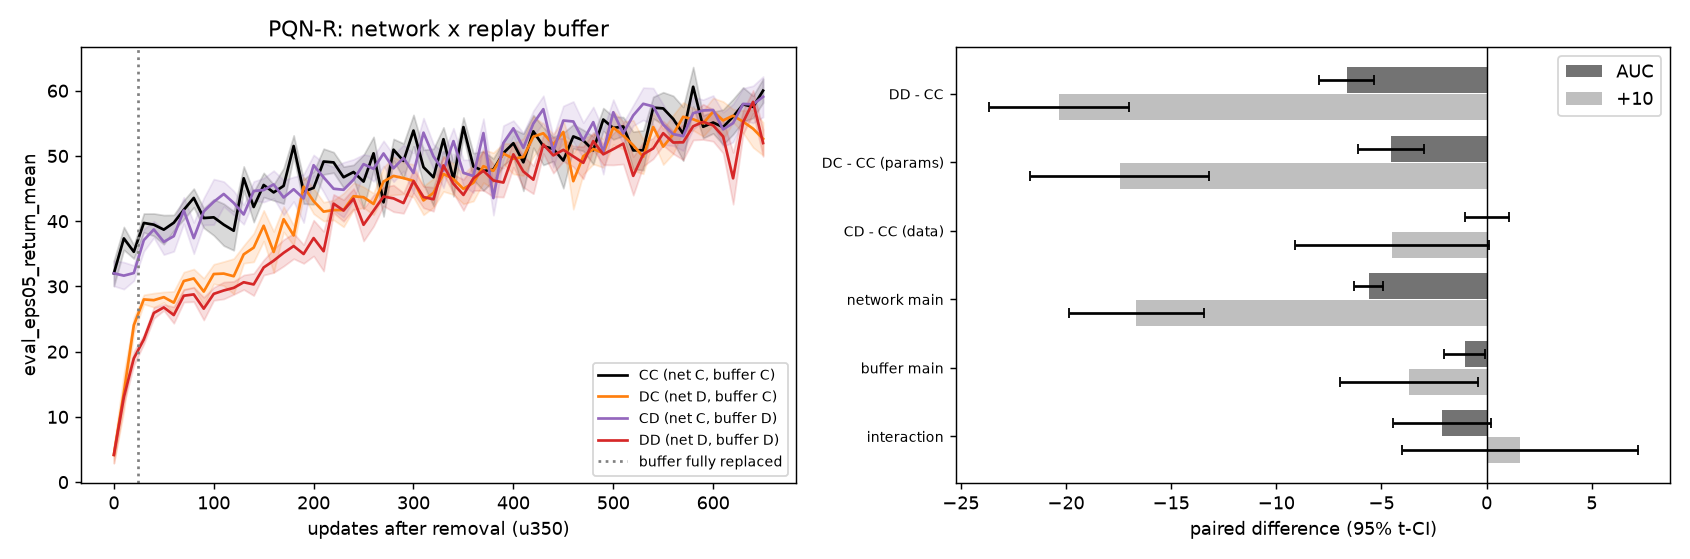
\includegraphics[width=\linewidth]{figures/p6_surgery_pqnr_n12.png}
\caption{PQN-R network $\times$ buffer surgery with a 100k buffer ($n=12$).}
\end{figure}

\begin{figure}[h]
\centering
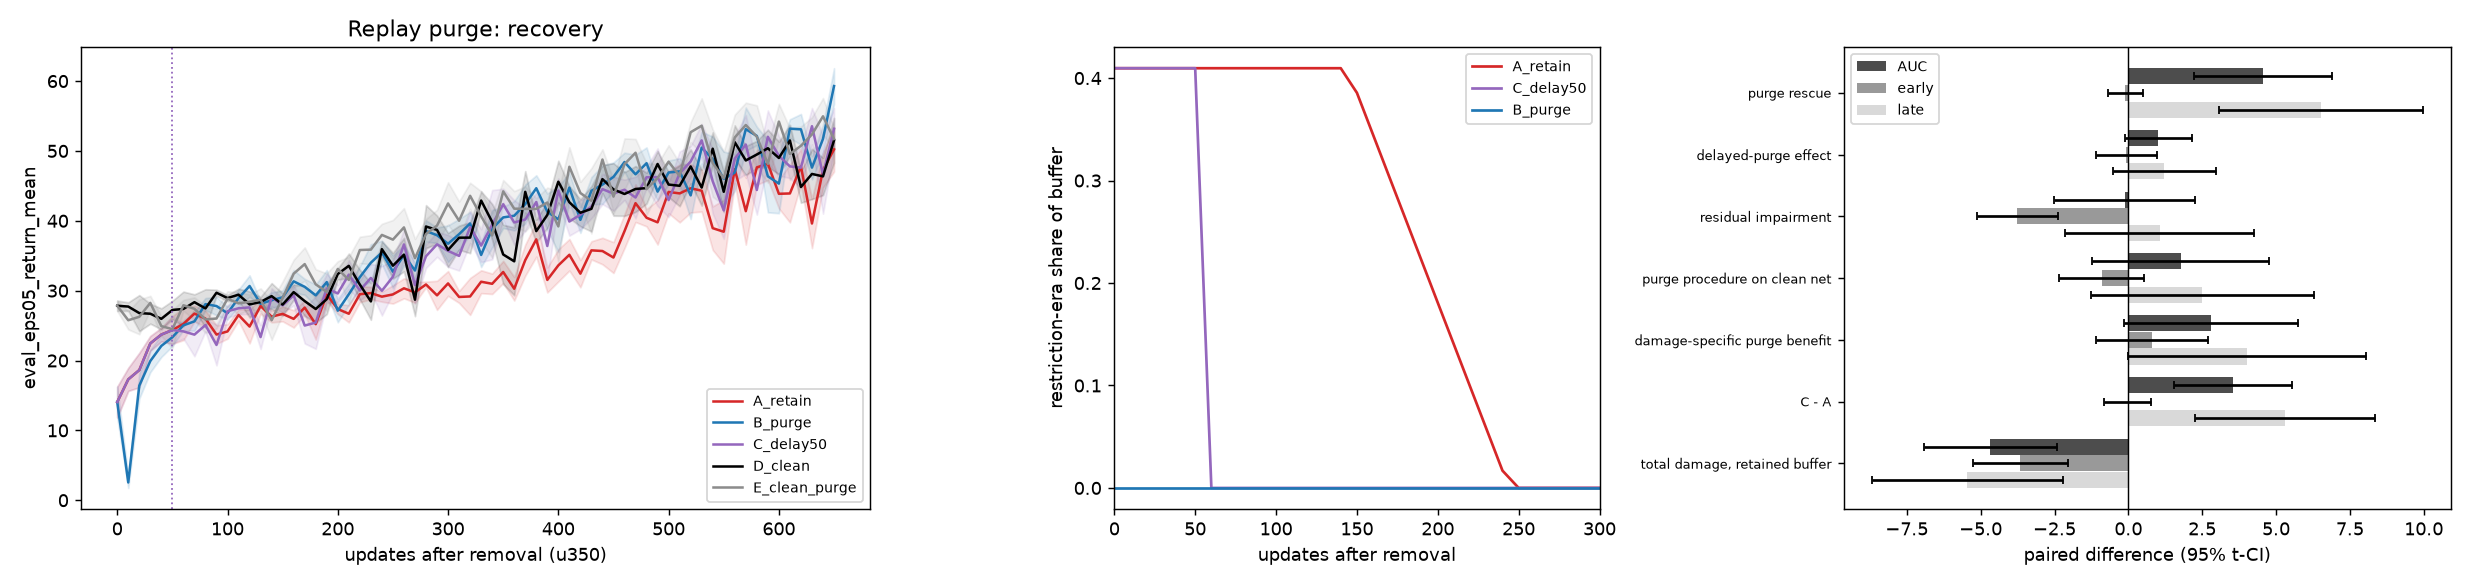
\includegraphics[width=\linewidth]{figures/p6_purge.png}
\caption{Rung 1: full replay purge ($n=8$). A: retain; B: purge at removal; C: purge delayed by 50 updates; D: clean agent; E: clean agent with purge.}
\end{figure}

\begin{figure}[h]
\centering
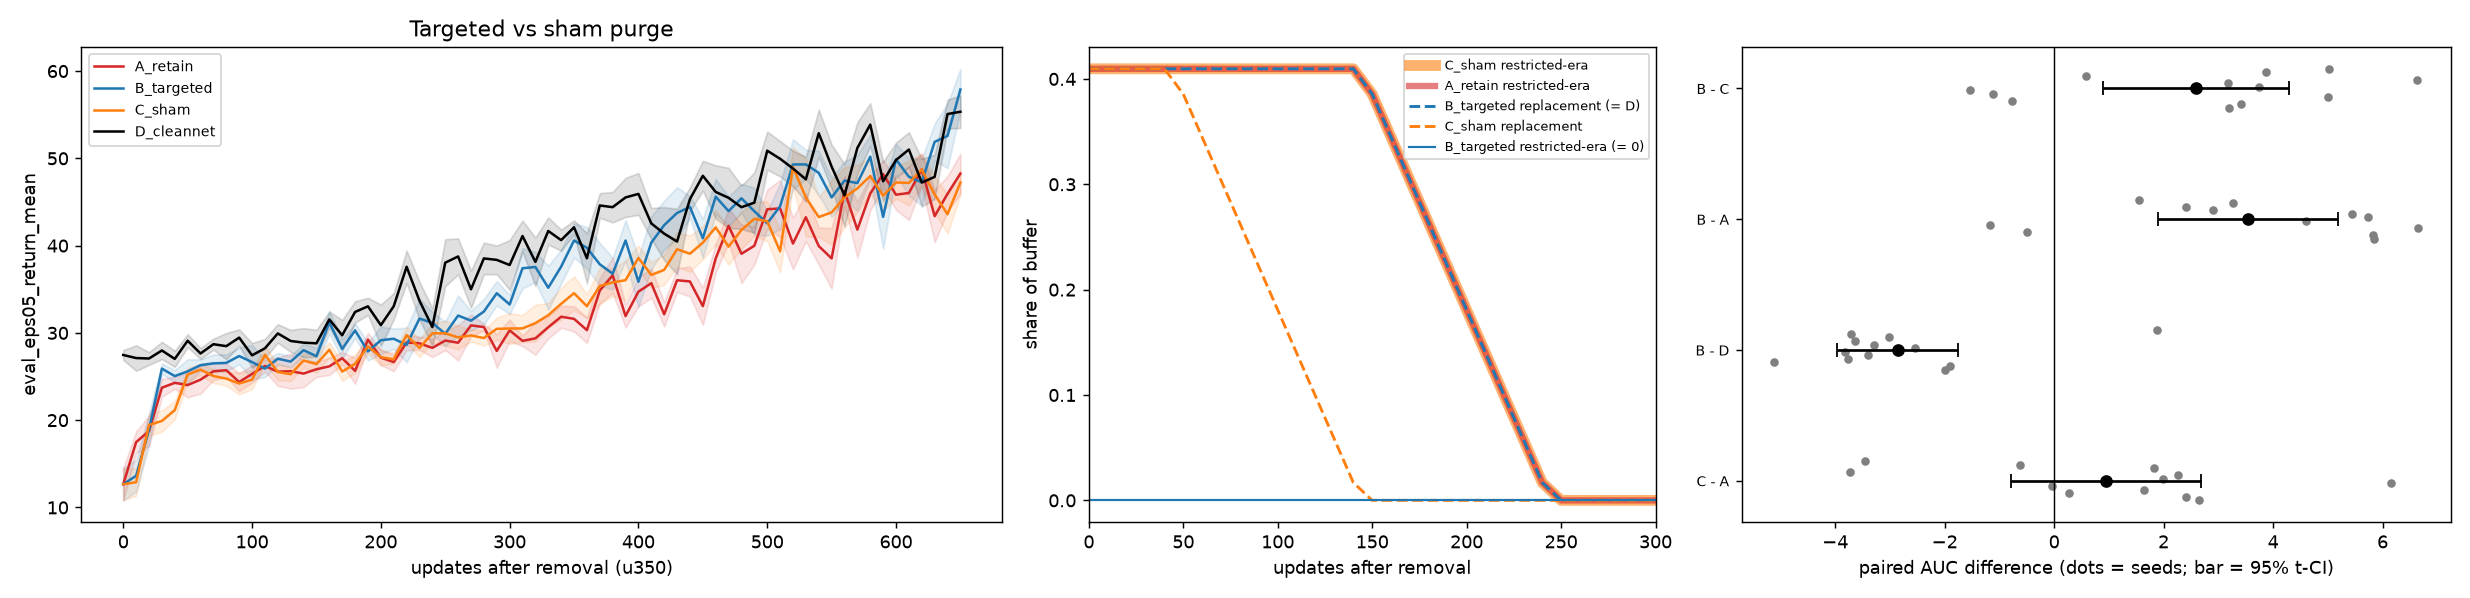
\includegraphics[width=\linewidth]{figures/p6b_targeted.png}
\caption{Rung 2: targeted purge of restriction-era rows vs.\ an age-nearest sham ($n=12$).}
\end{figure}

\begin{figure}[h]
\centering
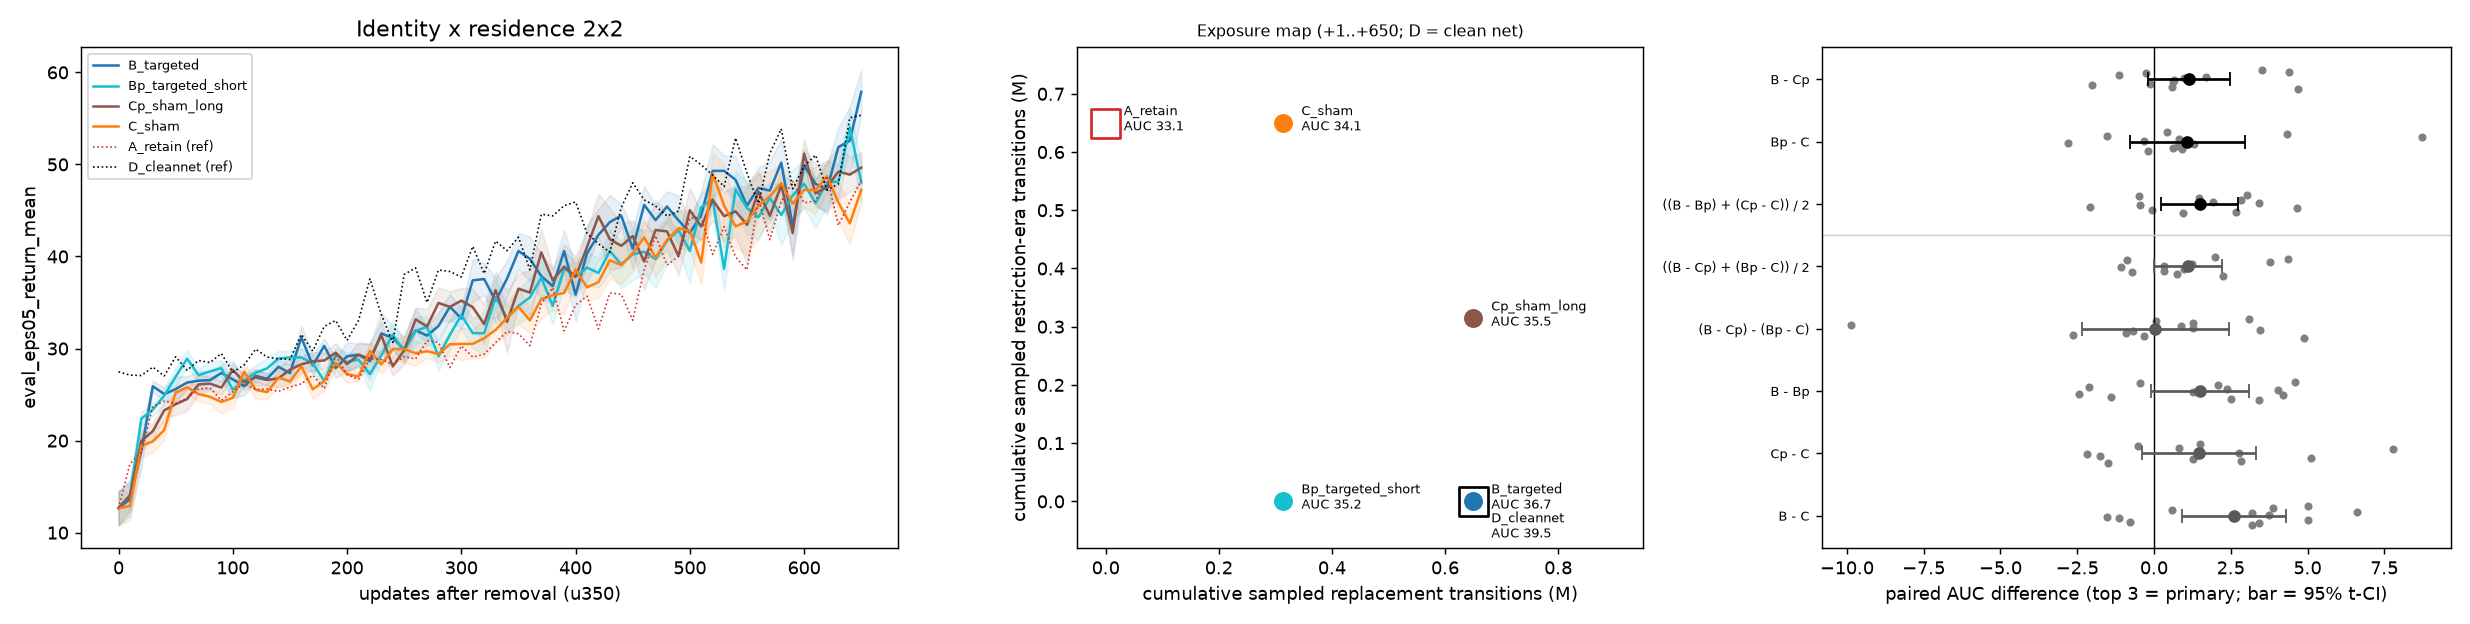
\includegraphics[width=\linewidth]{figures/p6c_2x2.png}
\caption{Rung 3: identity $\times$ residence $2\times2$ design ($n=12$).}
\end{figure}

\begin{figure}[h]
\centering
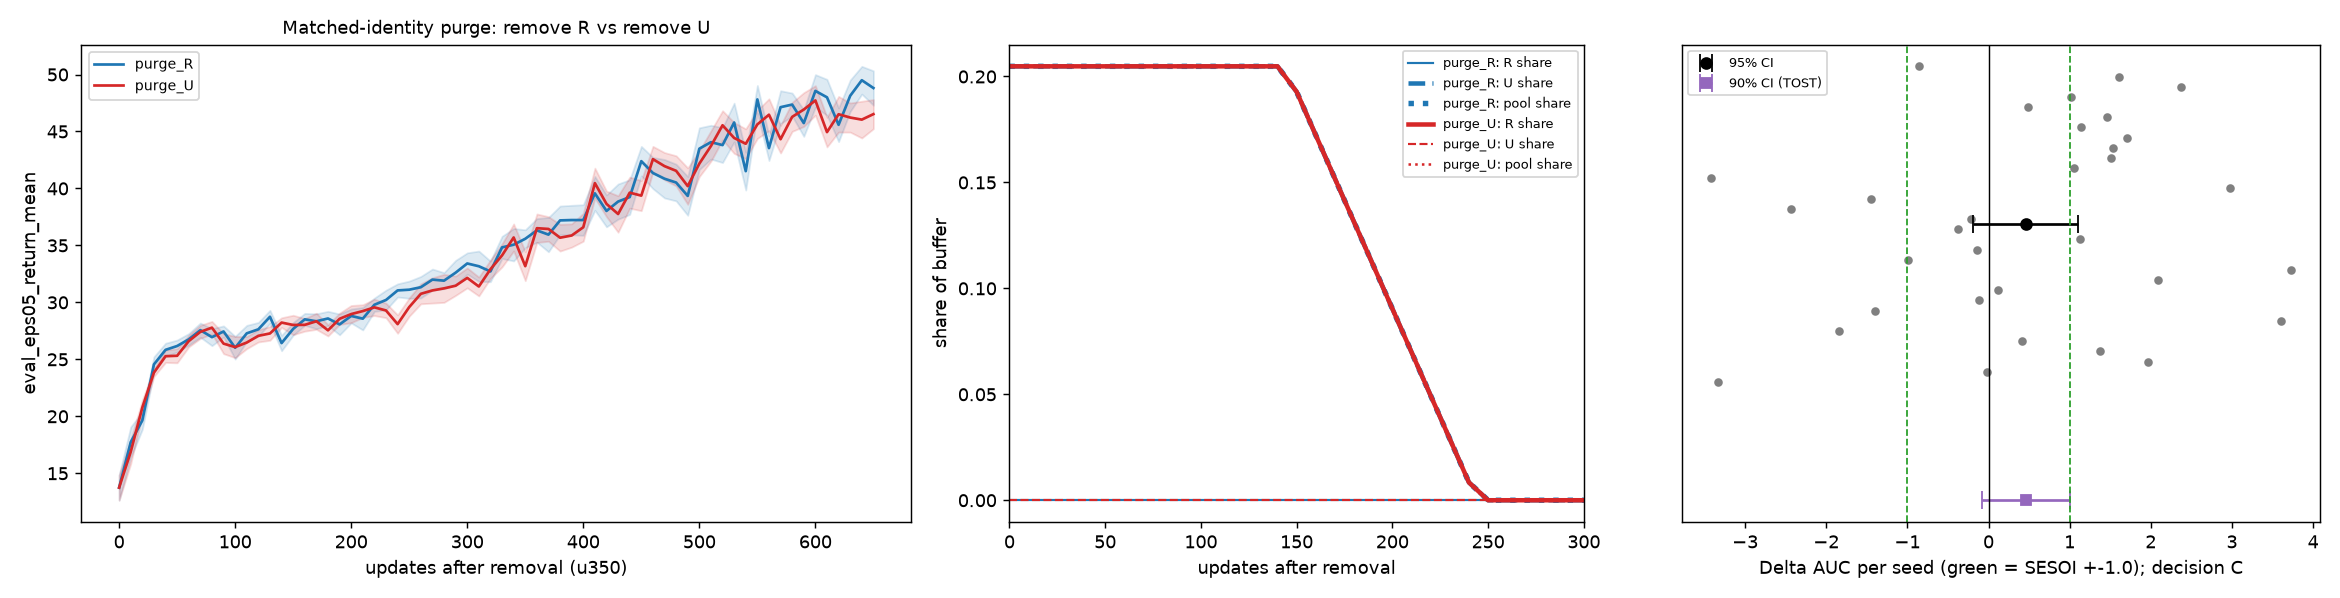
\includegraphics[width=\linewidth]{figures/p6d_idswap.png}
\caption{Rung 4: matched-identity purge ($n=32$) with the pre-registered equivalence margin.}
\end{figure}

\begin{figure}[h]
\centering
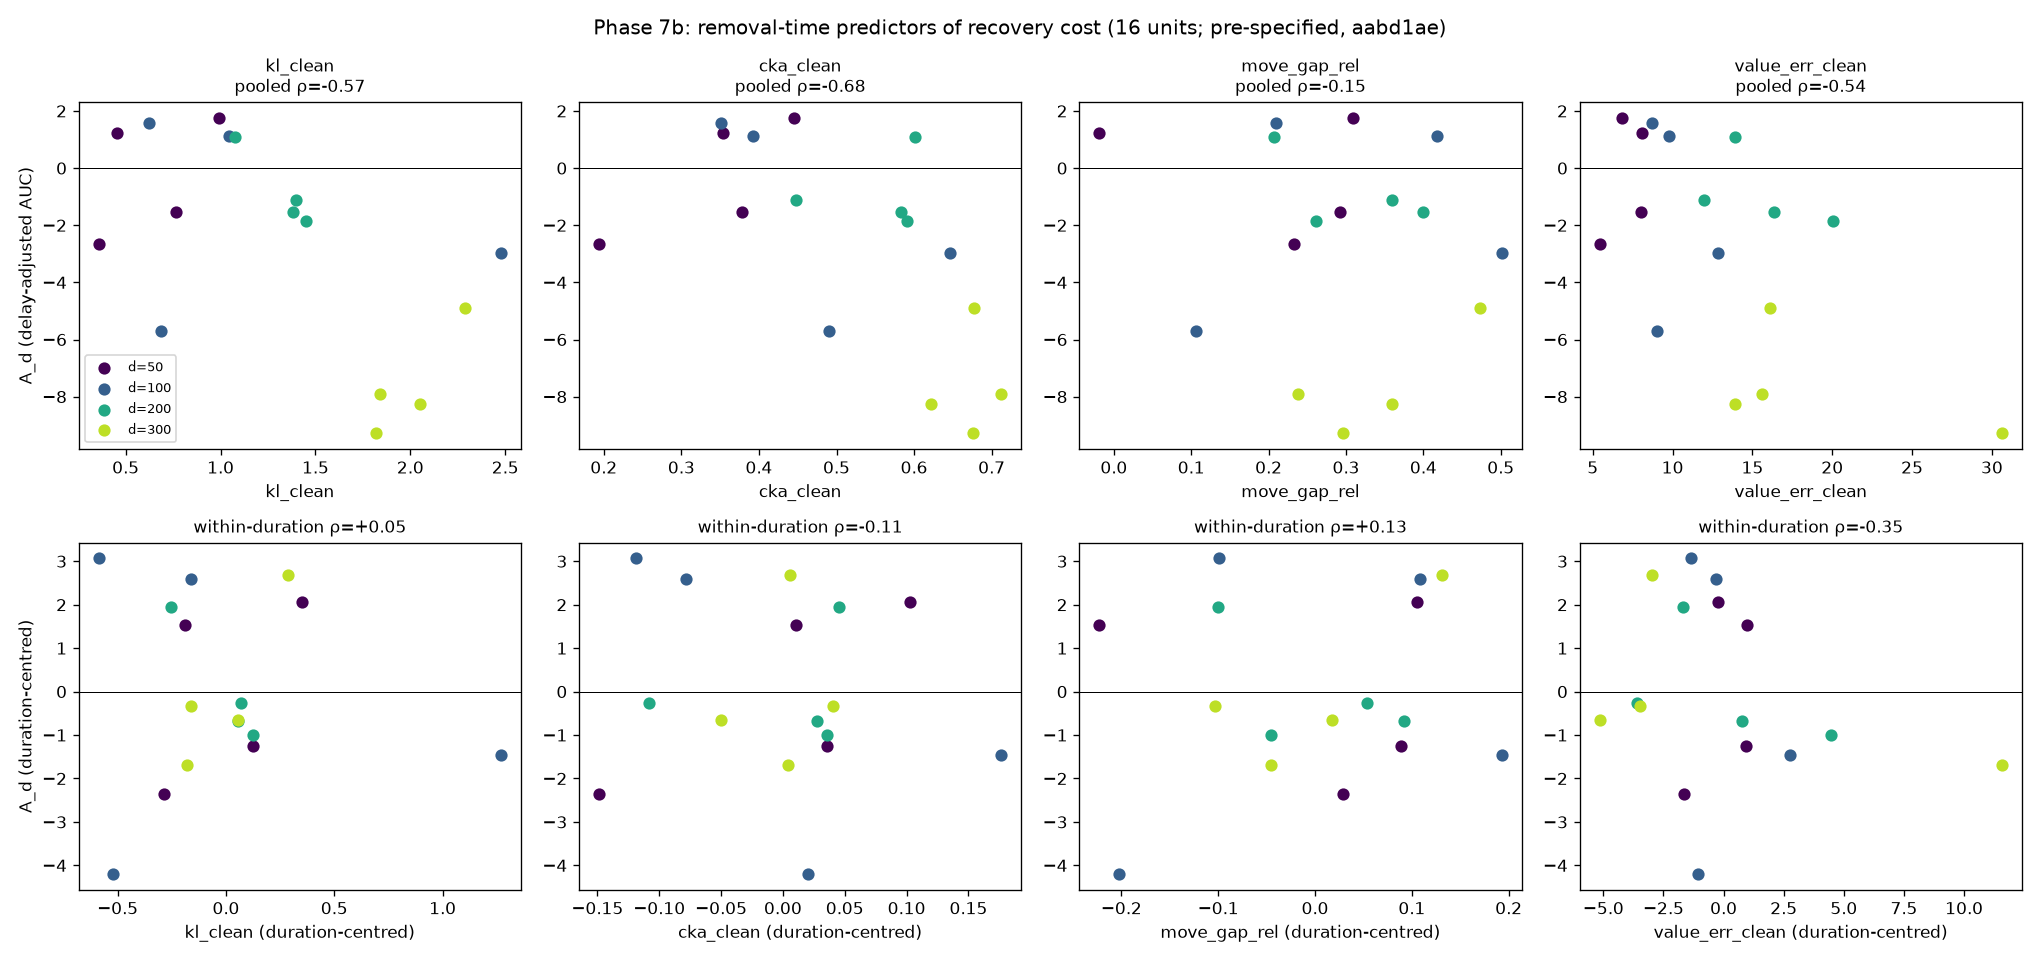
\includegraphics[width=\linewidth]{figures/p7b_predictors.png}
\caption{Phase 7b: pre-specified removal-time predictors against recovery cost. Pooled associations follow restriction length; within-duration associations were not detected ($n=4$ per duration).}
\end{figure}

\end{document}
